\documentclass[oneside,a4paper,14pt]{extarticle}
\usepackage[T1,T2A,TU]{fontenc}
\usepackage[a4paper,letterpaper,top=20mm,bottom=20mm,left=20mm,right=10mm]{geometry}
\usepackage[russian]{babel}
\usepackage{textcomp}
\usepackage{indentfirst}
\usepackage{graphicx}
\usepackage{mwe}
\usepackage{wrapfig}
\usepackage{caption}
\usepackage{amsmath}
\usepackage{amsfonts}
\usepackage{amsthm}
\usepackage{amssymb}
\usepackage[all]{xy}
\usepackage[breaklinks]{hyperref}
\usepackage{titlesec}
\usepackage{verbatim, fancyvrb}

\titleformat{\section} % Настройка формата заголовков секций
{\normalsize\bfseries} % Устанавливает размер шрифта на нормальный и делает его жирным
{\thesection} % Указывает, что номер секции будет отображаться перед заголовком
{1em} % Устанавливает расстояние между номером секции и заголовком в 1em
{} % Дополнительные параметры.

\titleformat{\subsection} % Настройка формата заголовков подсекций
{\normalsize\bfseries} % Устанавливает размер шрифта на нормальный и делает его жирным
{\thesubsection} % Указывает, что номер подсекции будет отображаться перед заголовком
{1em} % Устанавливает расстояние между номером подсекции и заголовком в 1em
{} % Дополнительные параметры.

\titleformat{\subsubsection} % Настройка формата заголовков подподсекций
{\normalsize\bfseries} % Устанавливает размер шрифта на нормальный и делает его жирным
{\thesubsection} % Указывает, что номер подподсекции будет отображаться перед заголовком
{1em} % Устанавливает расстояние между номером подподсекции и заголовком в 1em
{} % Дополнительные параметры.

\renewcommand\baselinestretch{1.45}\normalsize %межстр интервал
\setlength{\parindent}{1.25cm} %длина отступа нового абзаца

\begin{document}
\newpage
\thispagestyle{empty}
\begin{center}
	МИНИСТЕРСТВО НАУКИ И ВЫСШЕГО ОБРАЗОВАНИЯ\\
	РОССИЙСКОЙ ФЕДЕРАЦИИ
	ФЕДЕРАЛЬНОЕ ГОСУДАРСТВЕННОЕ БЮДЖЕТНОЕ\\
	ОБРАЗОВАТЕЛЬНОЕ
	УЧРЕЖДЕНИЕ ВЫСШЕГО ОБРАЗОВАНИЯ\\
	«ВЯТСКИЙ ГОСУДАРСТВЕННЫЙ УНИВЕРСИТЕТ»\\
	Институт математики и информационных систем\\
	Факультет автоматики и вычислительной техники\\
	Кафедра электронных вычислительных машин
\end{center}
\vspace{20mm}

\begin{center}
	Отчёт по лабораторной работе №1\\
	по дисциплине\\
	<<Программирование>>\\
\end{center}
\vspace{55mm}

Выполнил студент гр. ИВТб-1301-05-00 \hspace{5mm} \rule[-0,5mm]{30mm}{0.15mm}\,/Черкасов А. А./


Руководитель зав. кафедры ЭВМ \hfill  \rule[-0,5mm]{30mm}{0.15mm}\,/Долженкова М. Л./

\vfill
\begin{center}
	Киров\\
	2024
\end{center}

\newpage\thispagestyle{plain}

\section*{Цель}

\sloppy Цель работы: изучение и применение основ программирования на языках Pascal и C через выполнение практических заданий, направленных на развитие навыков алгоритмического мышления, освоение синтаксиса языков, а также на решение задач, связанных с обработкой данных и реализацией алгоритмов.

\section*{Задания}

\begin{enumerate}
	\item \textbf{Наибольшая последовательность.} \\
	      Среди введенных N чисел определить длину максимальной возрастающей последовательности.\\

	      \textbf{Формат ввода.} \\
	      В первой строке задается число N - количество чисел в последовательности. Во второй строке через пробел задаются числа последовательности. \\

	      \textbf{Формат вывода.} \\
	      Выводится целое число соответствующее максимальной длине возрастающей последовательности.\\
	      $$
		      \begin{tabular}{ll}
			      \textbf{Ввод}  & \textbf{Вывод} \\
			      \hline
			      7              & 4              \\
			      1 2 3 -1 3 4 8 &                \\
			      \hline
		      \end{tabular}
	      $$
	      \newpage
	\item \textbf{Сумма M младших.} \\
	      Для заданных натуральных чисел M и N. Получить сумму M младших цифр числа N. \\

	      \textbf{Формат ввода.} \\
	      В первой строке вводится натуральное число $0 \leqslant N \leqslant 9999999$. Во второй - натуральное число M.\\

	      \textbf{Формат вывода.}\\
	      Выводится единственное число, соответствующие сумме M младших цифр.

	      $$
		      \begin{tabular}{ll}
			      \textbf{Ввод} & \textbf{Вывод} \\
			      \hline
			      3741762       & 15             \\
			      3             &                \\
			      \hline
		      \end{tabular}
	      $$

	\item \textbf{Красивое число.} \\
	      Будем называть трехзначное число "красивым", если полусумма его минимальной и максимальной цифры меньше оставшейся. Определите является ли введенное число "красивым".\\

	      \textbf{Формат ввода.} \\
	      В единственной строке задается трехзначное целое число.\\

	      \textbf{Формат вывода.}\\
	      Вывести "YES", если число "красивое" и "NO" в противном случае.\\
	      $$
		      \begin{tabular}{ll}
			      \textbf{Ввод} & \textbf{Вывод} \\
			      \hline
			      936           & NO             \\
			      \hline
			      570           & YES            \\
			      \hline
		      \end{tabular}
	      $$
	\item \textbf{Номер наименьшего.} \\
	      Среди произвольного количества целых чисел определить минимальный порядковый номер наименьшего из них.\\

	      \textbf{Формат ввода.} \\
	      В единственной строке задается набор целых чисел, заканчивающийся значением "0".\\

	      \textbf{Формат вывода.}\\
	      Целое число соответствующее номеру минимального числа в наборе (нумерация с 0)\\
	      $$
		      \begin{tabular}{ll}
			      \textbf{Ввод} & \textbf{Вывод} \\
			      \hline
			      -4 -5 5 -5 0  & 1              \\
			      \hline
		      \end{tabular}
	      $$
	\item \textbf{Про кирпич.} \\
	      В некоторой стене осталось не закрытым прямоугольное
	      отверстие размером А на В. Определить, проходит ли кирпич с
	      размерами x, y, z через это отверстие. \\

	      \textbf{Формат ввода.} \\
	      В единственной строке заданы пять натуральных чисед A , B, x,y,z.
	      Диапазон представления входных данных от 0 до 99999.\\

	      \textbf{Формат вывода.}\\
	      Вывести слово "Yes", если кирпич войдет в отверстие и "No" в противном случае.\\
	      $$
		      \begin{tabular}{ll}
			      \textbf{Ввод} & \textbf{Вывод} \\
			      \hline
			      7 6 8 1 1     & Yes            \\
			      \hline
			      2 6 8 3 2     & Yes            \\
			      \hline
		      \end{tabular}
	      $$
	\item \textbf{Площадь прямоугольника.} \\
	      Заданы координаты вершин прямоугольника со сторонами,
	      параллельными осям координат (x1,y1) и (x2,y2). Определить площадь части
	      прямоугольника, расположенной в первой координатной четверти. \\

	      \textbf{Формат ввода.} \\
	      В единственной строке вводятся 4 целых числа x1 y1 x2 y2 (через
	      пробел). Диапазон допустимых значений от -9999999 до 9999999\\

	      \textbf{Формат вывода.}\\
	      В единственной строке выводится целое число, соответствующее
	      искомой площади.\\
	      $$
		      \begin{tabular}{ll}
			      \textbf{Ввод}            & \textbf{Вывод} \\
			      \hline
			      78943 84425 62396 -20854 & 1396980475     \\
			      \hline
		      \end{tabular}
	      $$
	\item \textbf{Чередование.} \\
	      Дана непустая последовательность ненулевых целых чисел. Определить,
	      сколько раз в этой последовательности меняется знак. Например, в
	      последовательности 1, -3, 8, 1, -5 знак меняется 3 раза. \pagebreak

	      \textbf{Формат ввода.} \\
	      В первой строке задается N-е количество чисел в
	      последовательности. Во второй строке - целые числа составляющие
	      последовательность через пробел.\\

	      \textbf{Формат вывода.}\\
	      В единственной строке выводится целое число. \\
	      $$
		      \begin{tabular}{ll}
			      \textbf{Ввод}           & \textbf{Вывод} \\
			      \hline
			      10                      & 5              \\
			      1 2 3 -3 -2 2 2 -1 5 -8 &                \\
			      \hline
		      \end{tabular}
	      $$
	\item \textbf{Языковые группы.} \\
	      Необходимо протестировать группу из N человек. Каждый из них
	      вводит: 1 --- если он изучал английский язык, 2 --- если немецкий, 3 ---
	      если французский, 0 --- если не изучал никакой. Определите, сколько
	      человек в каждой языковой группе.\\

	      \textbf{Формат ввода.} \\
	      В первой строке вводится натуральное число N - количество опрошенных. В следующих N строках указывается возможный ответ (3,2,1,0).\\

	      \textbf{Формат вывода.}\\
	      В первой строке вывести число тех, кто изучал английский язык во второй - если немецкий, в третьей – французский.\\
	      \pagebreak
	\item \textbf{Счастливый билетик.} \\
	      В катушке с автобусными билетами (номер билета шестизначный)
	      меньший номер билета n, больший m. Определить количество счастливых
	      билетов.\\

	      \textbf{Формат ввода.} \\
	      В единственной строке вводятся через пробел два натуральных числа
	      N и M соответствующие шестизначному номеру первого и последнего билетов в
	      катушке.\\

	      \textbf{Формат вывода.}\\
	      В строке выводится одно целое число, количество счастливых билетов.\\
	      $$
		      \begin{tabular}{ll}
			      \textbf{Ввод} & \textbf{Вывод} \\
			      \hline
			      111111 111112 & 1              \\
			      \hline
		      \end{tabular}
	      $$
	\item \textbf{Хорошая группа.}\\
	      В университете на потоке учатся M групп. Каждый месяц декан проводит конкурс на "хорошую" группу. Для этого оценивается число пропущенных занятий каждым студентом группы. и рассчитывается среднее значение по группе Nm, где m номер группы. Если минимальное число пропусков N1, N2, N3, N4...Nm меньше 10, то на потоке «Есть хорошая группа». Помогите декану провести конкурс. Если хорошая группа найдется выведите сообщение «The good group» и укажите ее номер. Если такой группы нет выведете "No".

	      \textbf{Формат ввода.} \\
	      В первой строке вводится натуральное число M - количество групп в потоке Далее в каждой следующей строке натуральное число K-количество студентов в группе, а затем через пробел число пропусков каждого студента.\\

	      \textbf{Формат вывода.}\\
	      В единственной строке выводится The good group и через пробел натуральное число ее номер (группы нумеруются в порядке ввода начиная с единицы). Если хорошая группа не найдена в строке выводится слово No.\\
	      $$
		      \begin{tabular}{ll}
			      \textbf{Ввод}                            & \textbf{Вывод}   \\
			      \hline
			      4                                        & The good group 3 \\
			      13 10 19 9 13 14 16 14 10 10 5 8 14 3    &                  \\
			      2 17 6                                   &                  \\
			      15 10 2 9 10 10 11 4 10 4 11 1 1 10 6 12 &                  \\
			      \hline
		      \end{tabular}
	      $$
	\item \textbf{Точка пересечения.}\\
	      Заданы $k_1, b_1, k_2, b_2$ и e $(e > 0)$. Определить, находится ли точка пересечения прямых заданных уравнениями. $y = k_1 \cdot x + b_1$ и $y = k_2 \cdot x + b_2$ на расстоянии не более e от начала координат. \\

	      \textbf{Формат ввода.} \\
	      В строке через пробел вводятся 5 целых чисел $k_1, b_1, k_2, b_2$ и е соответсвенно. \\

	      \textbf{Формат вывода.}\\
	      Выводится сообщение Yes, если точка соответствует условию и No в противном случае.
	      $$
		      \begin{tabular}{ll}
			      \textbf{Ввод} & \textbf{Вывод} \\
			      \hline
			      1 0 3 -2 2    & Yes            \\
			      \hline
			      -3 1 6 -35 9  & No             \\
			      \hline
		      \end{tabular}
	      $$
	      \pagebreak

	\item \textbf{Совершенное число.}\\
	      Дано натуральное число n. Проверить, является ли оно совершенным (число называется совершенным, если оно равно сумме всех своих делителей).\\

	      \textbf{Формат ввода.} \\
	      В единственной строке задается целое число n.\\

	      \textbf{Формат вывода.} \\
	      Выводится сообщение YES, если число совершенное и NO в противном случае.\\
	      $$
		      \begin{tabular}{ll}
			      \textbf{Ввод} & \textbf{Вывод} \\
			      \hline
			      6             & YES            \\
			      \hline
			      5             & NO             \\
			      \hline
		      \end{tabular}
	      $$
\end{enumerate}
\section*{Вывод}
В ходе лабораторной работы были выработаны навыки алгоритмического мышления и решения задач, что позволило лучше понять принципы обработки данных и реализации алгоритмов. Выполнение практических заданий способствовало закреплению знаний о синтаксисе языков программирования и их применении.
\pagebreak

\begin{figure}
	\centering
	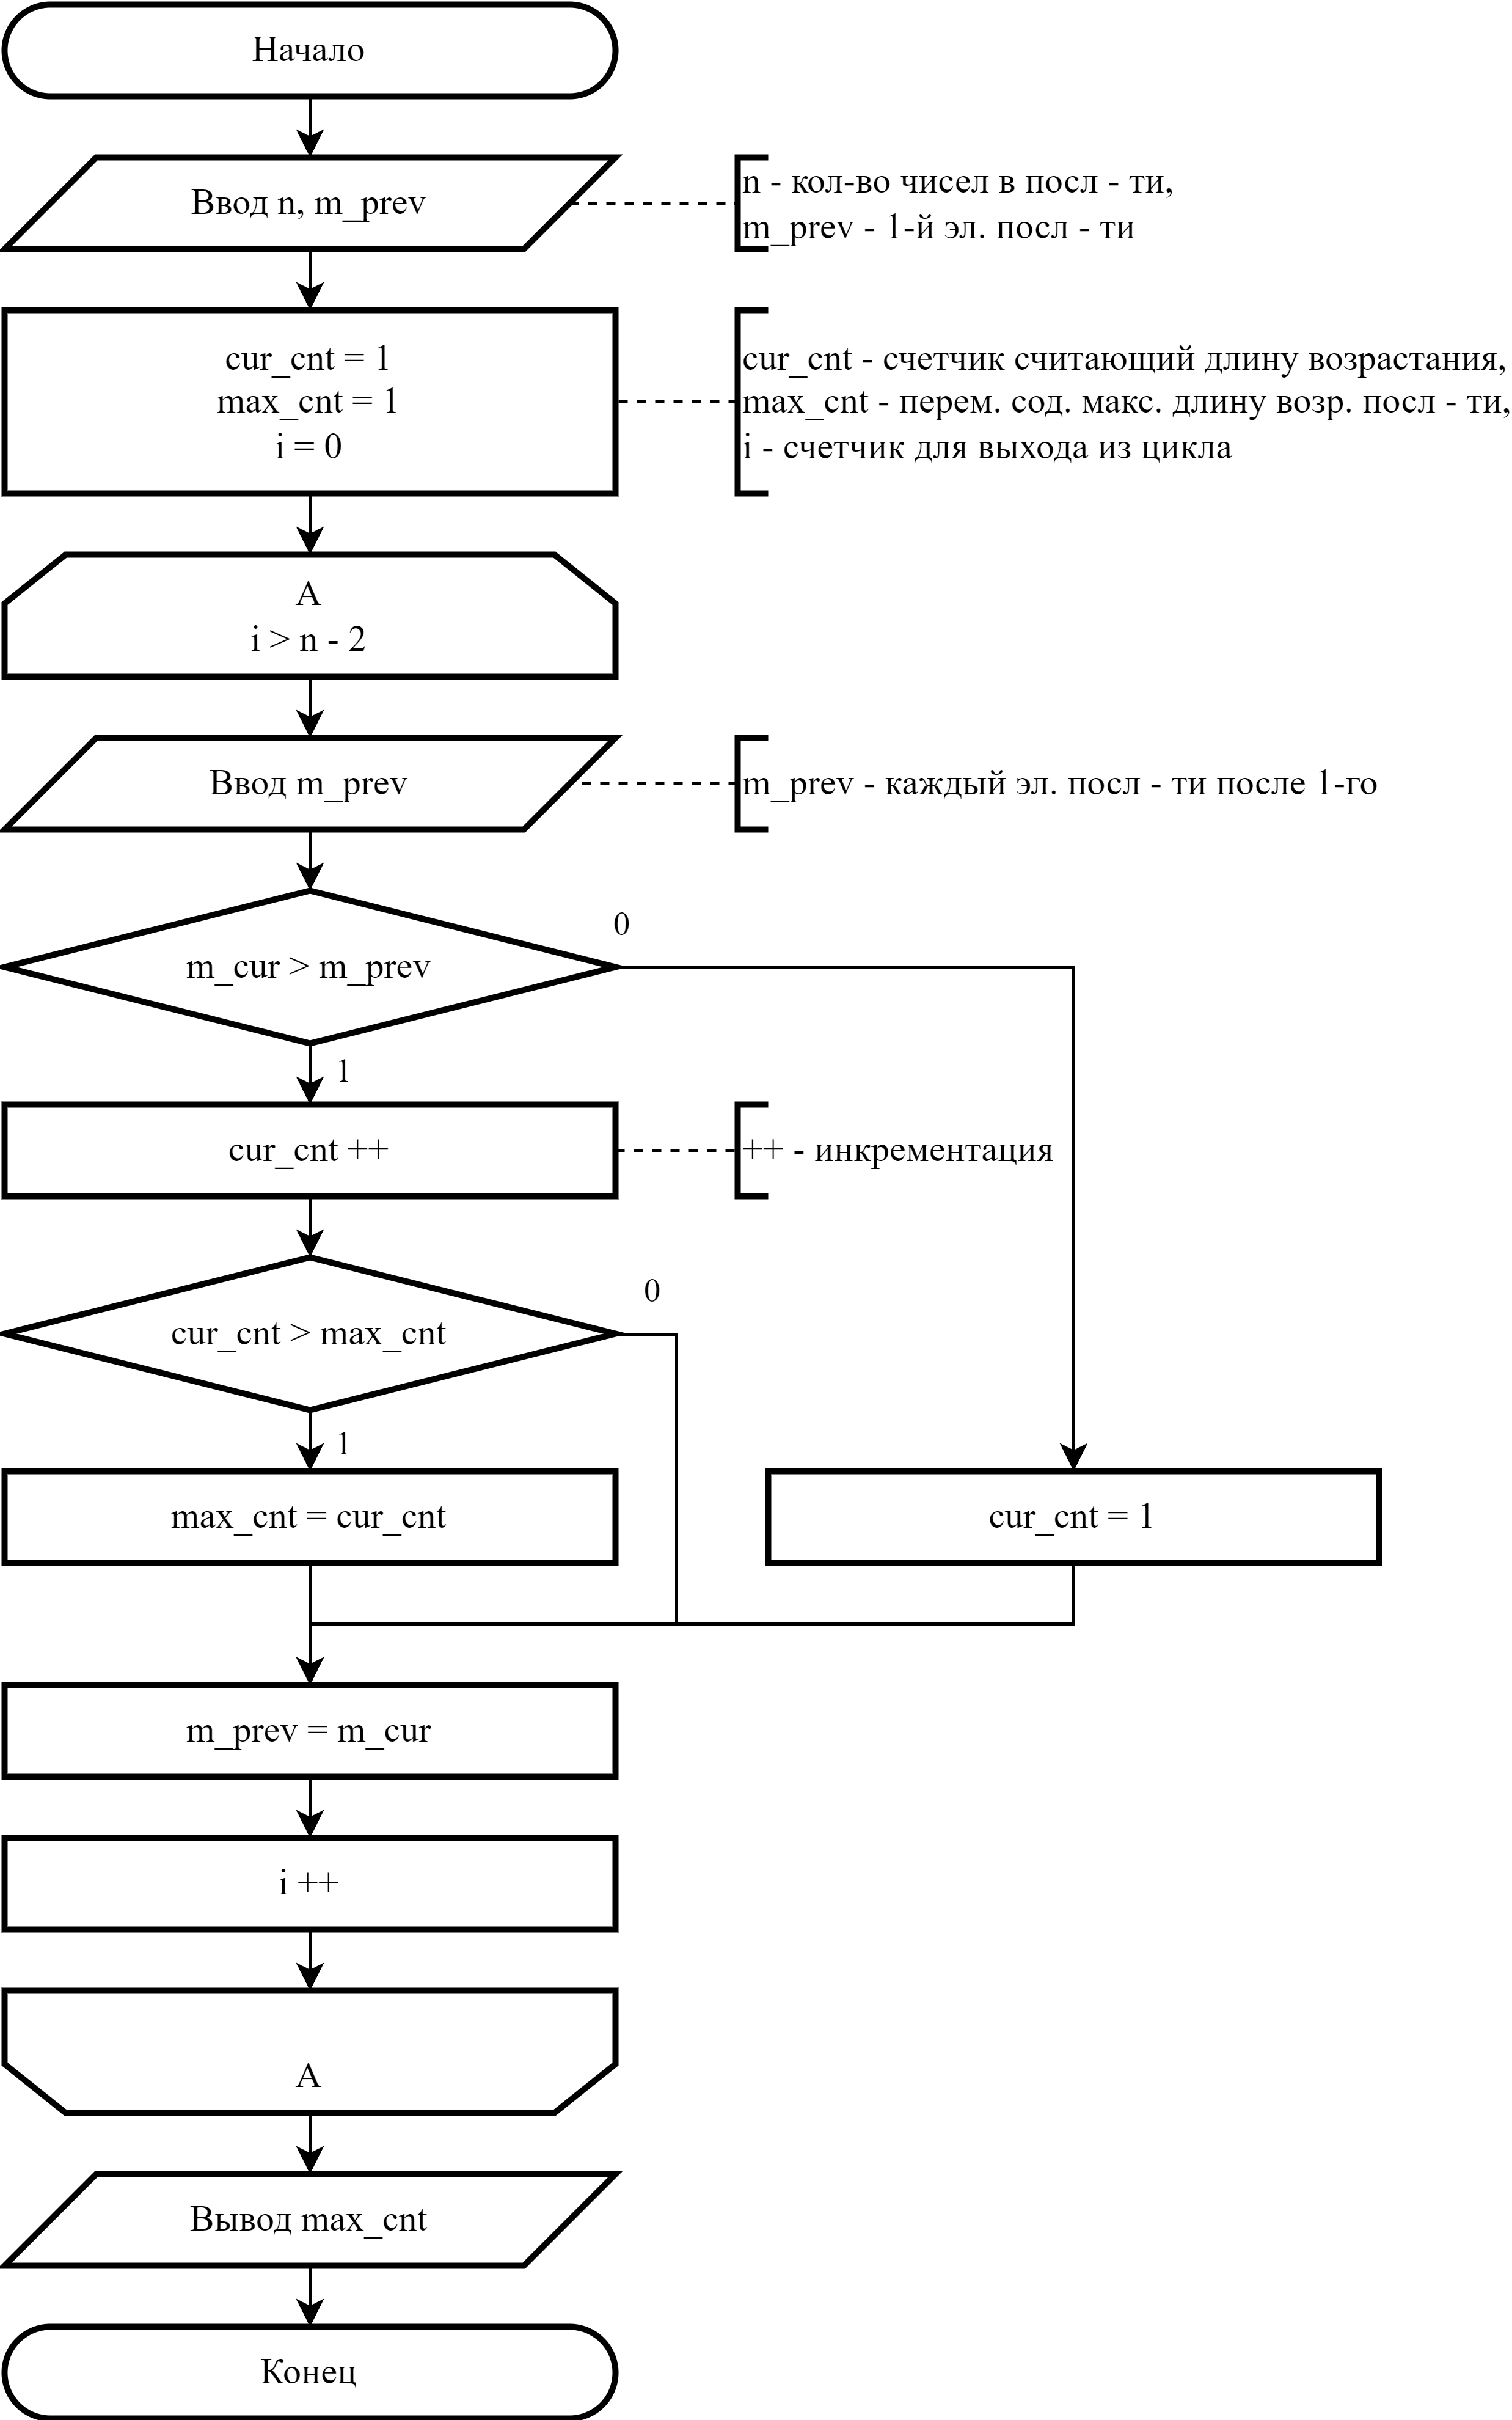
\includegraphics[height=0.9\textheight]{img/1-scheme.png} % Укажите путь к изображению
	\caption{Схема алгоритма решения Задания 1.} % Подпись к изображению
\end{figure}
\begin{figure}
	\centering
	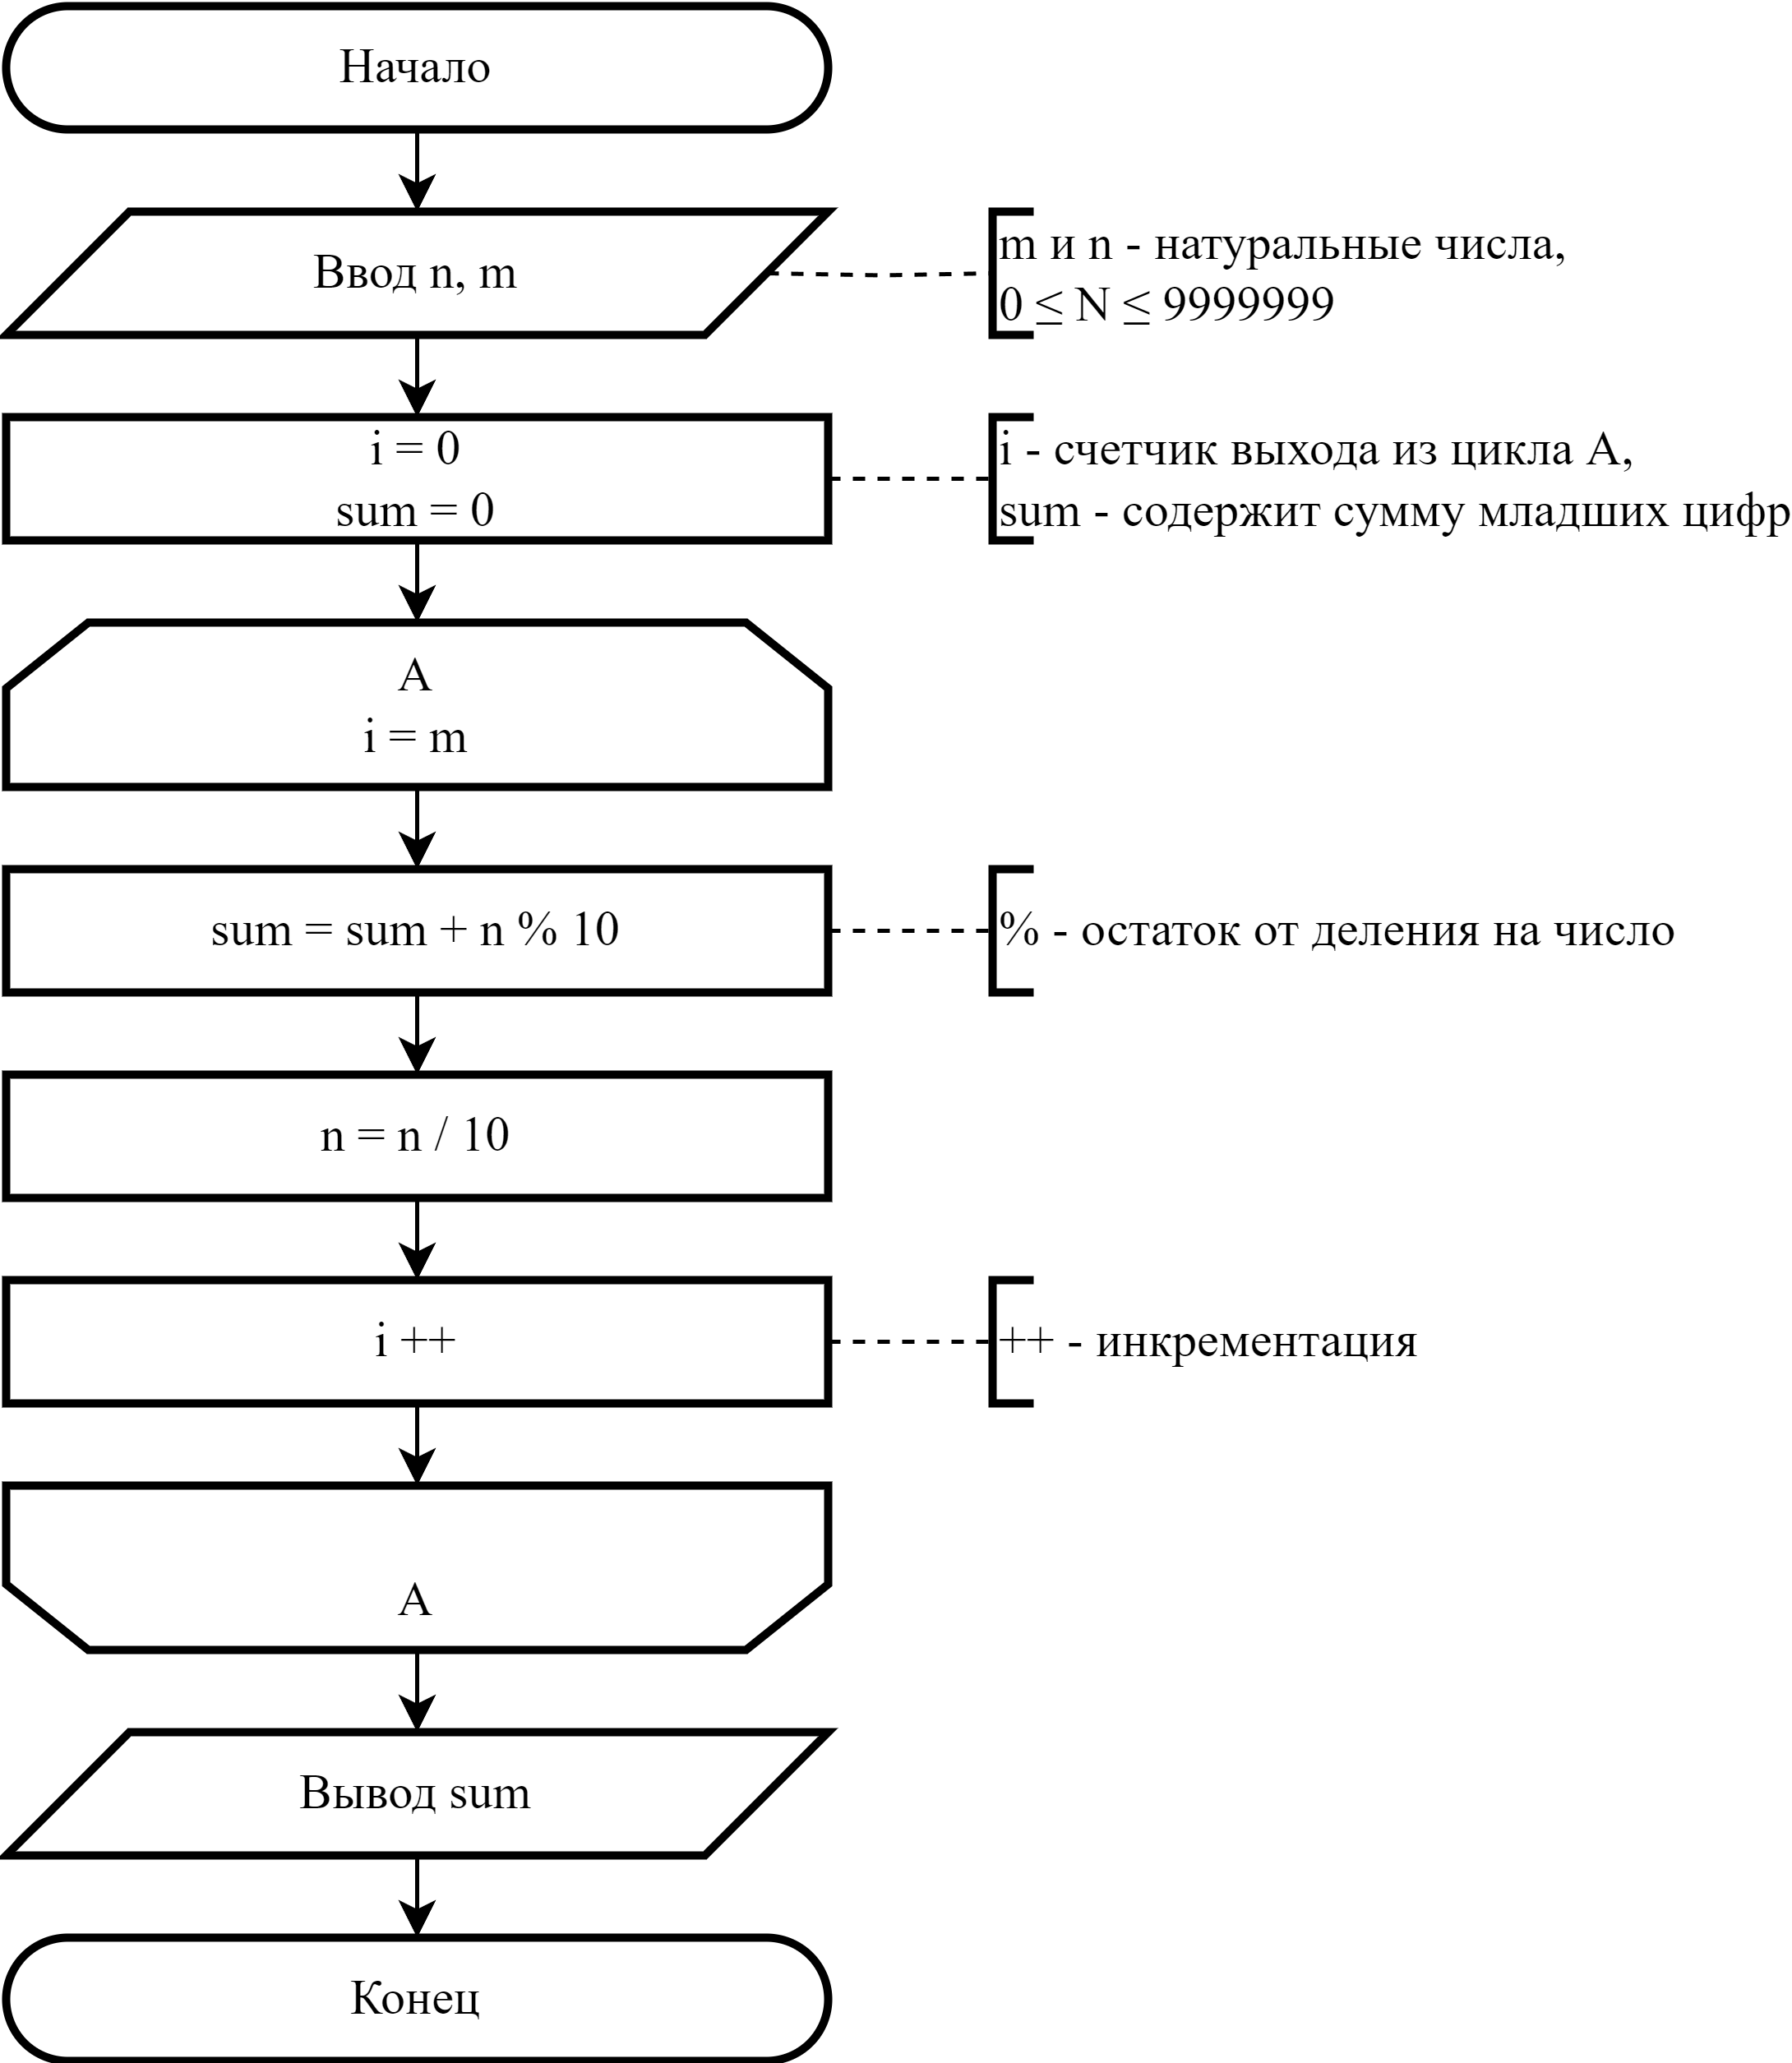
\includegraphics[width=0.65\textwidth]{img/2-scheme.png} % Укажите путь к изображению
	\caption{Схема алгоритма решения Задания 2.} % Подпись к изображению
\end{figure}
\begin{figure}
	\centering
	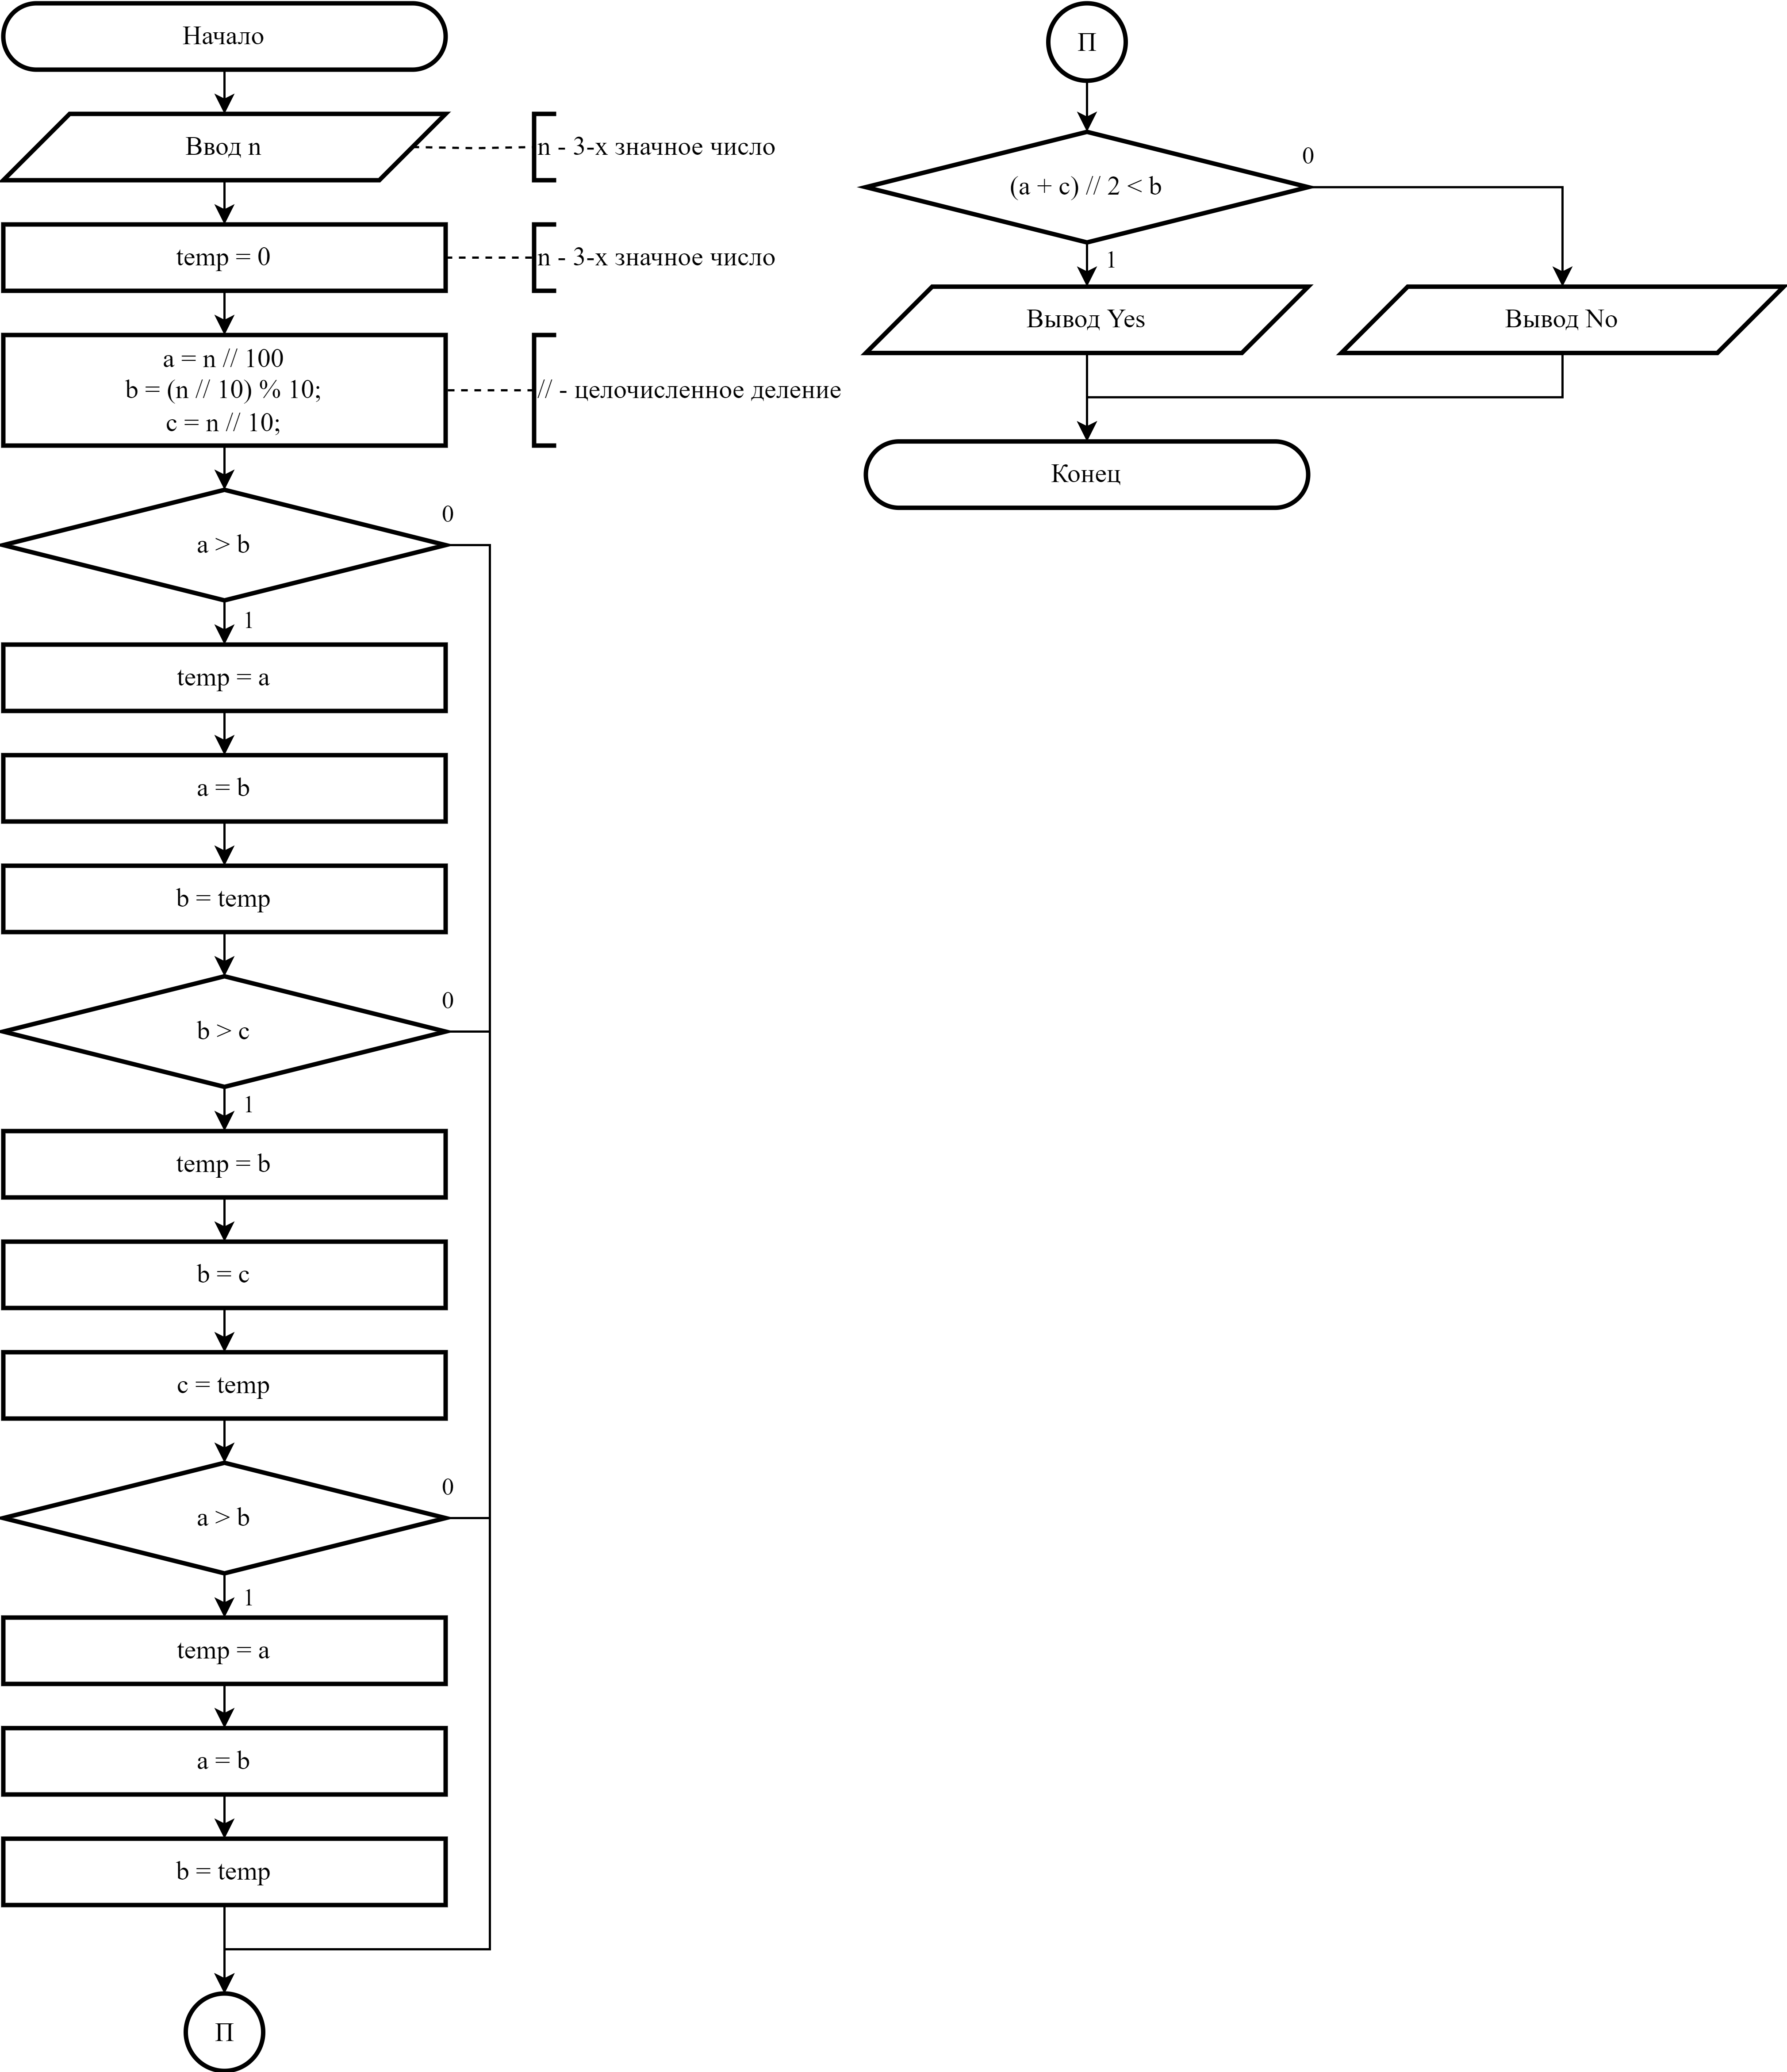
\includegraphics[width=\textwidth]{img/3-scheme.png} % Укажите путь к изображению
	\caption{Схема алгоритма решения Задания 3.} % Подпись к изображению
\end{figure}
\begin{figure}
	\centering
	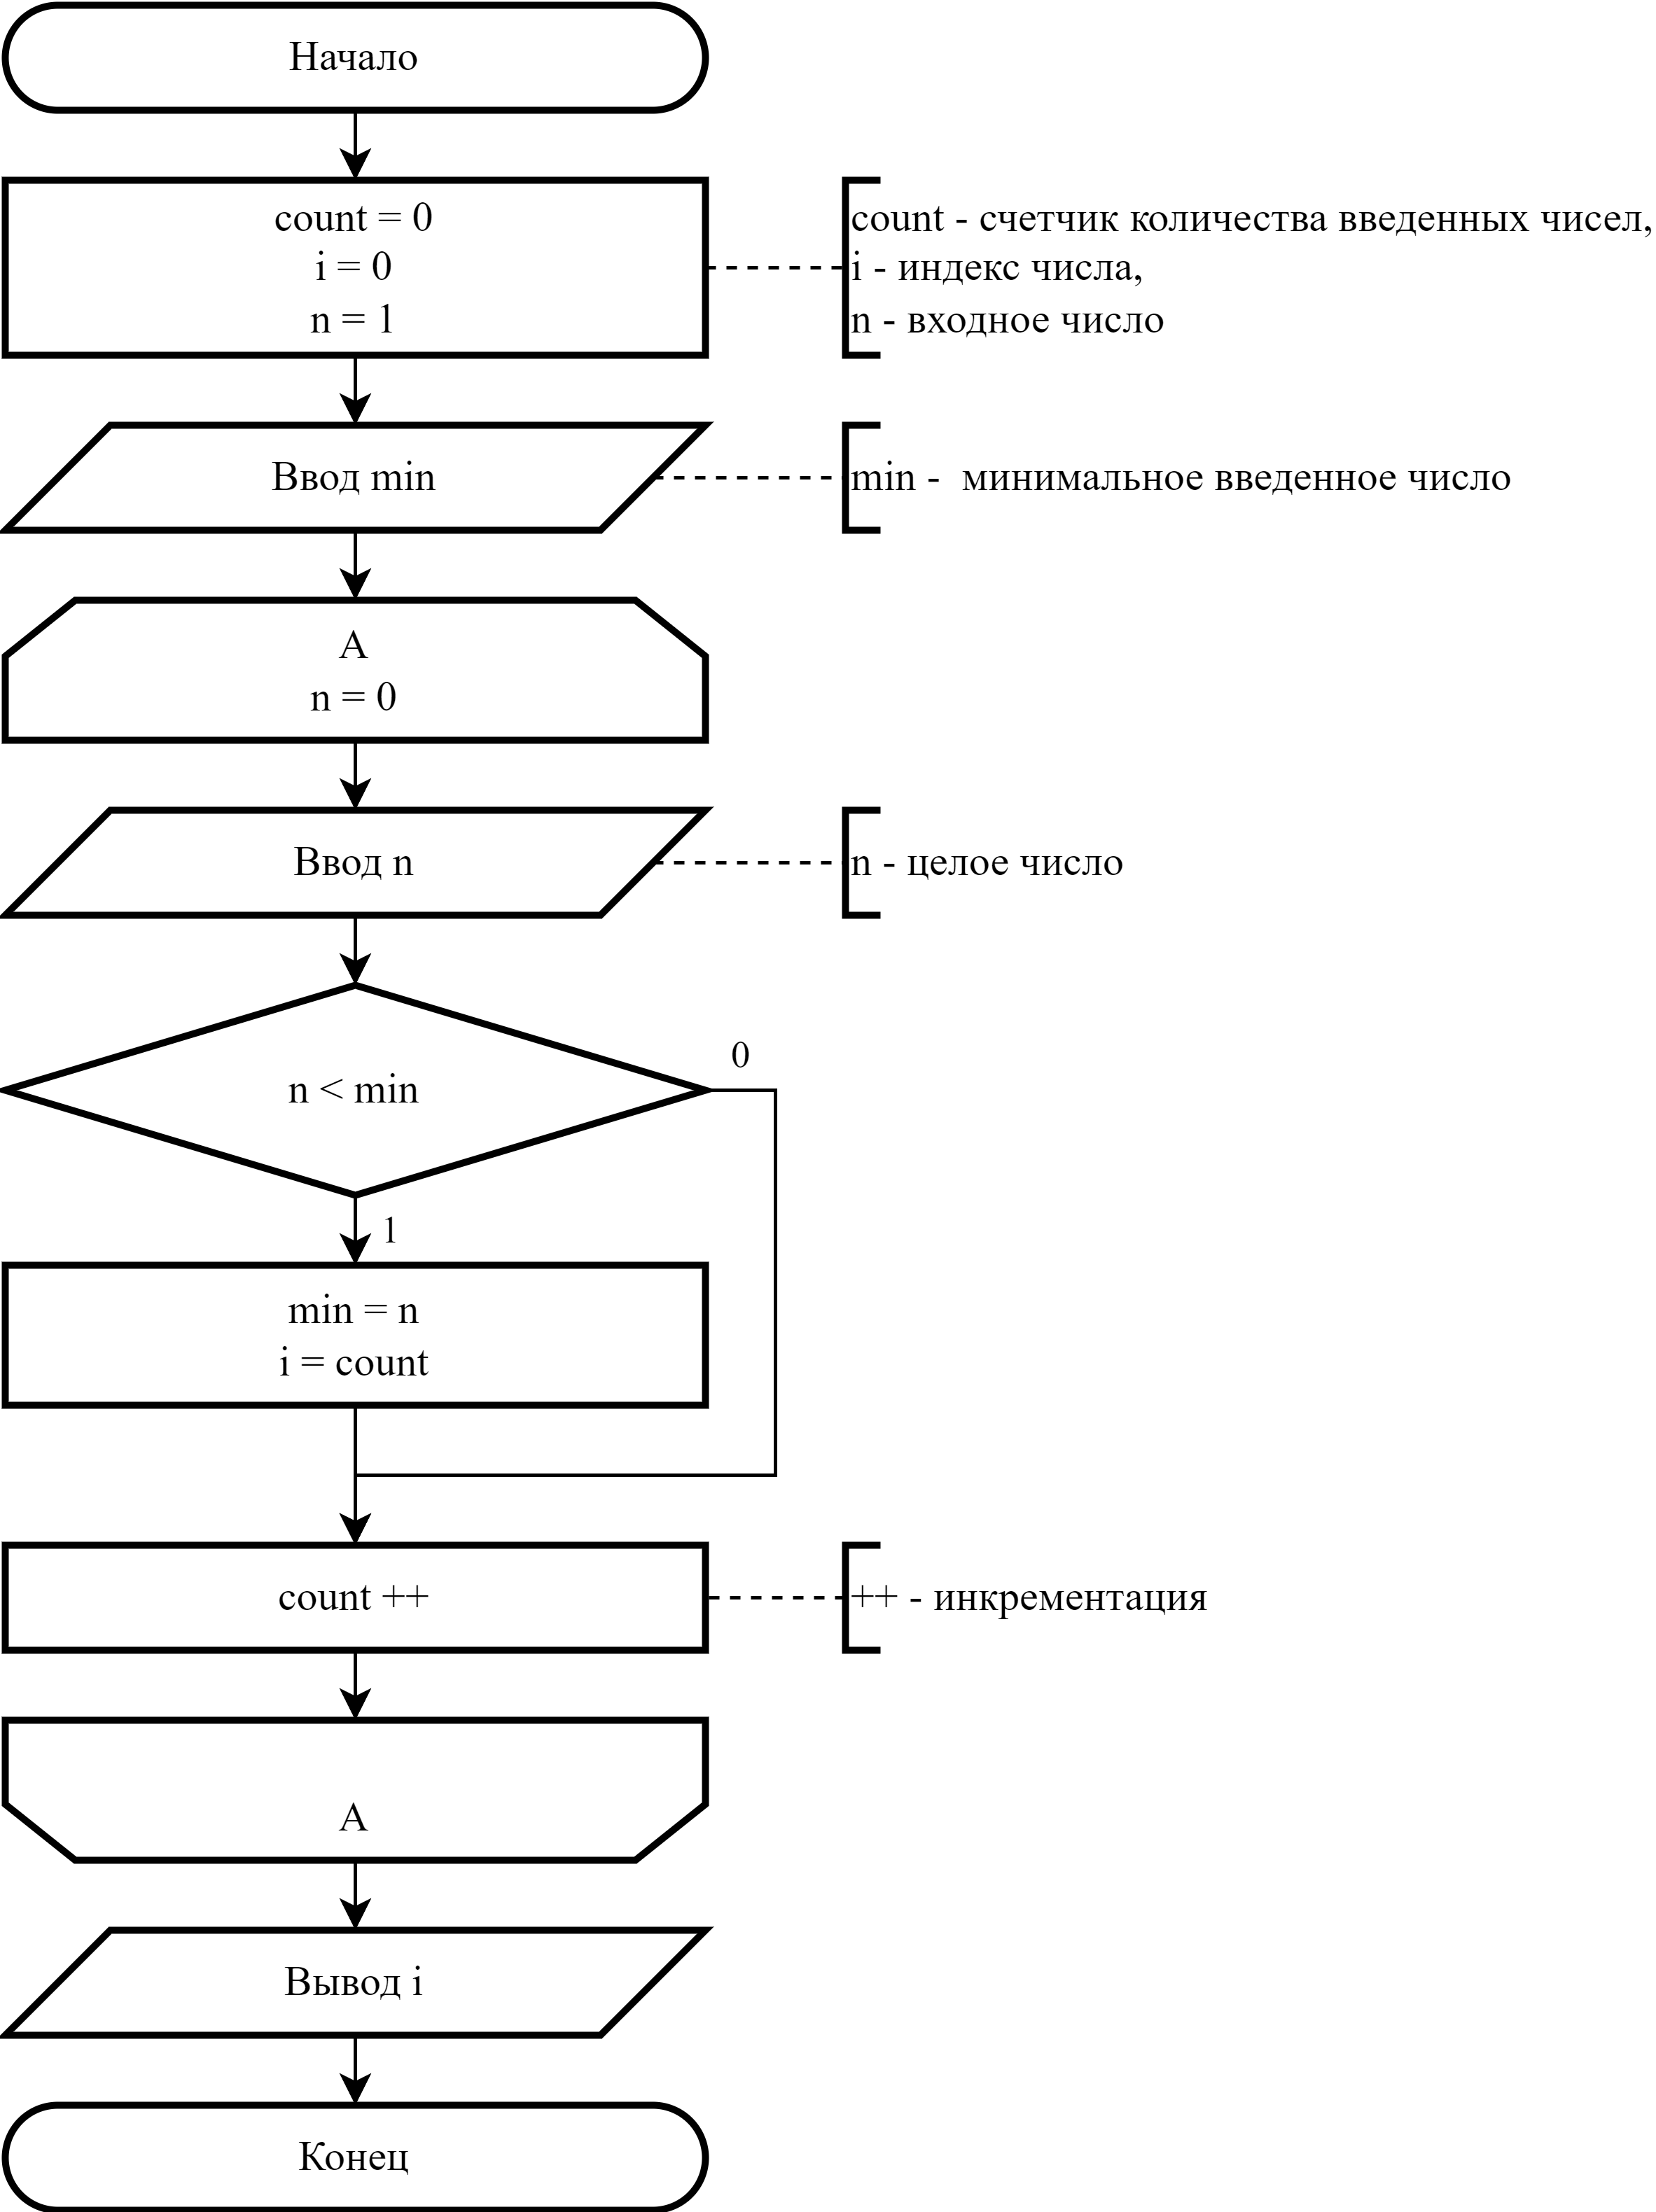
\includegraphics[width=0.75\textwidth]{img/4-scheme.png} % Укажите путь к изображению
	\caption{Схема алгоритма решения Задания 4.} % Подпись к изображению
\end{figure}
\begin{figure}
	\centering
	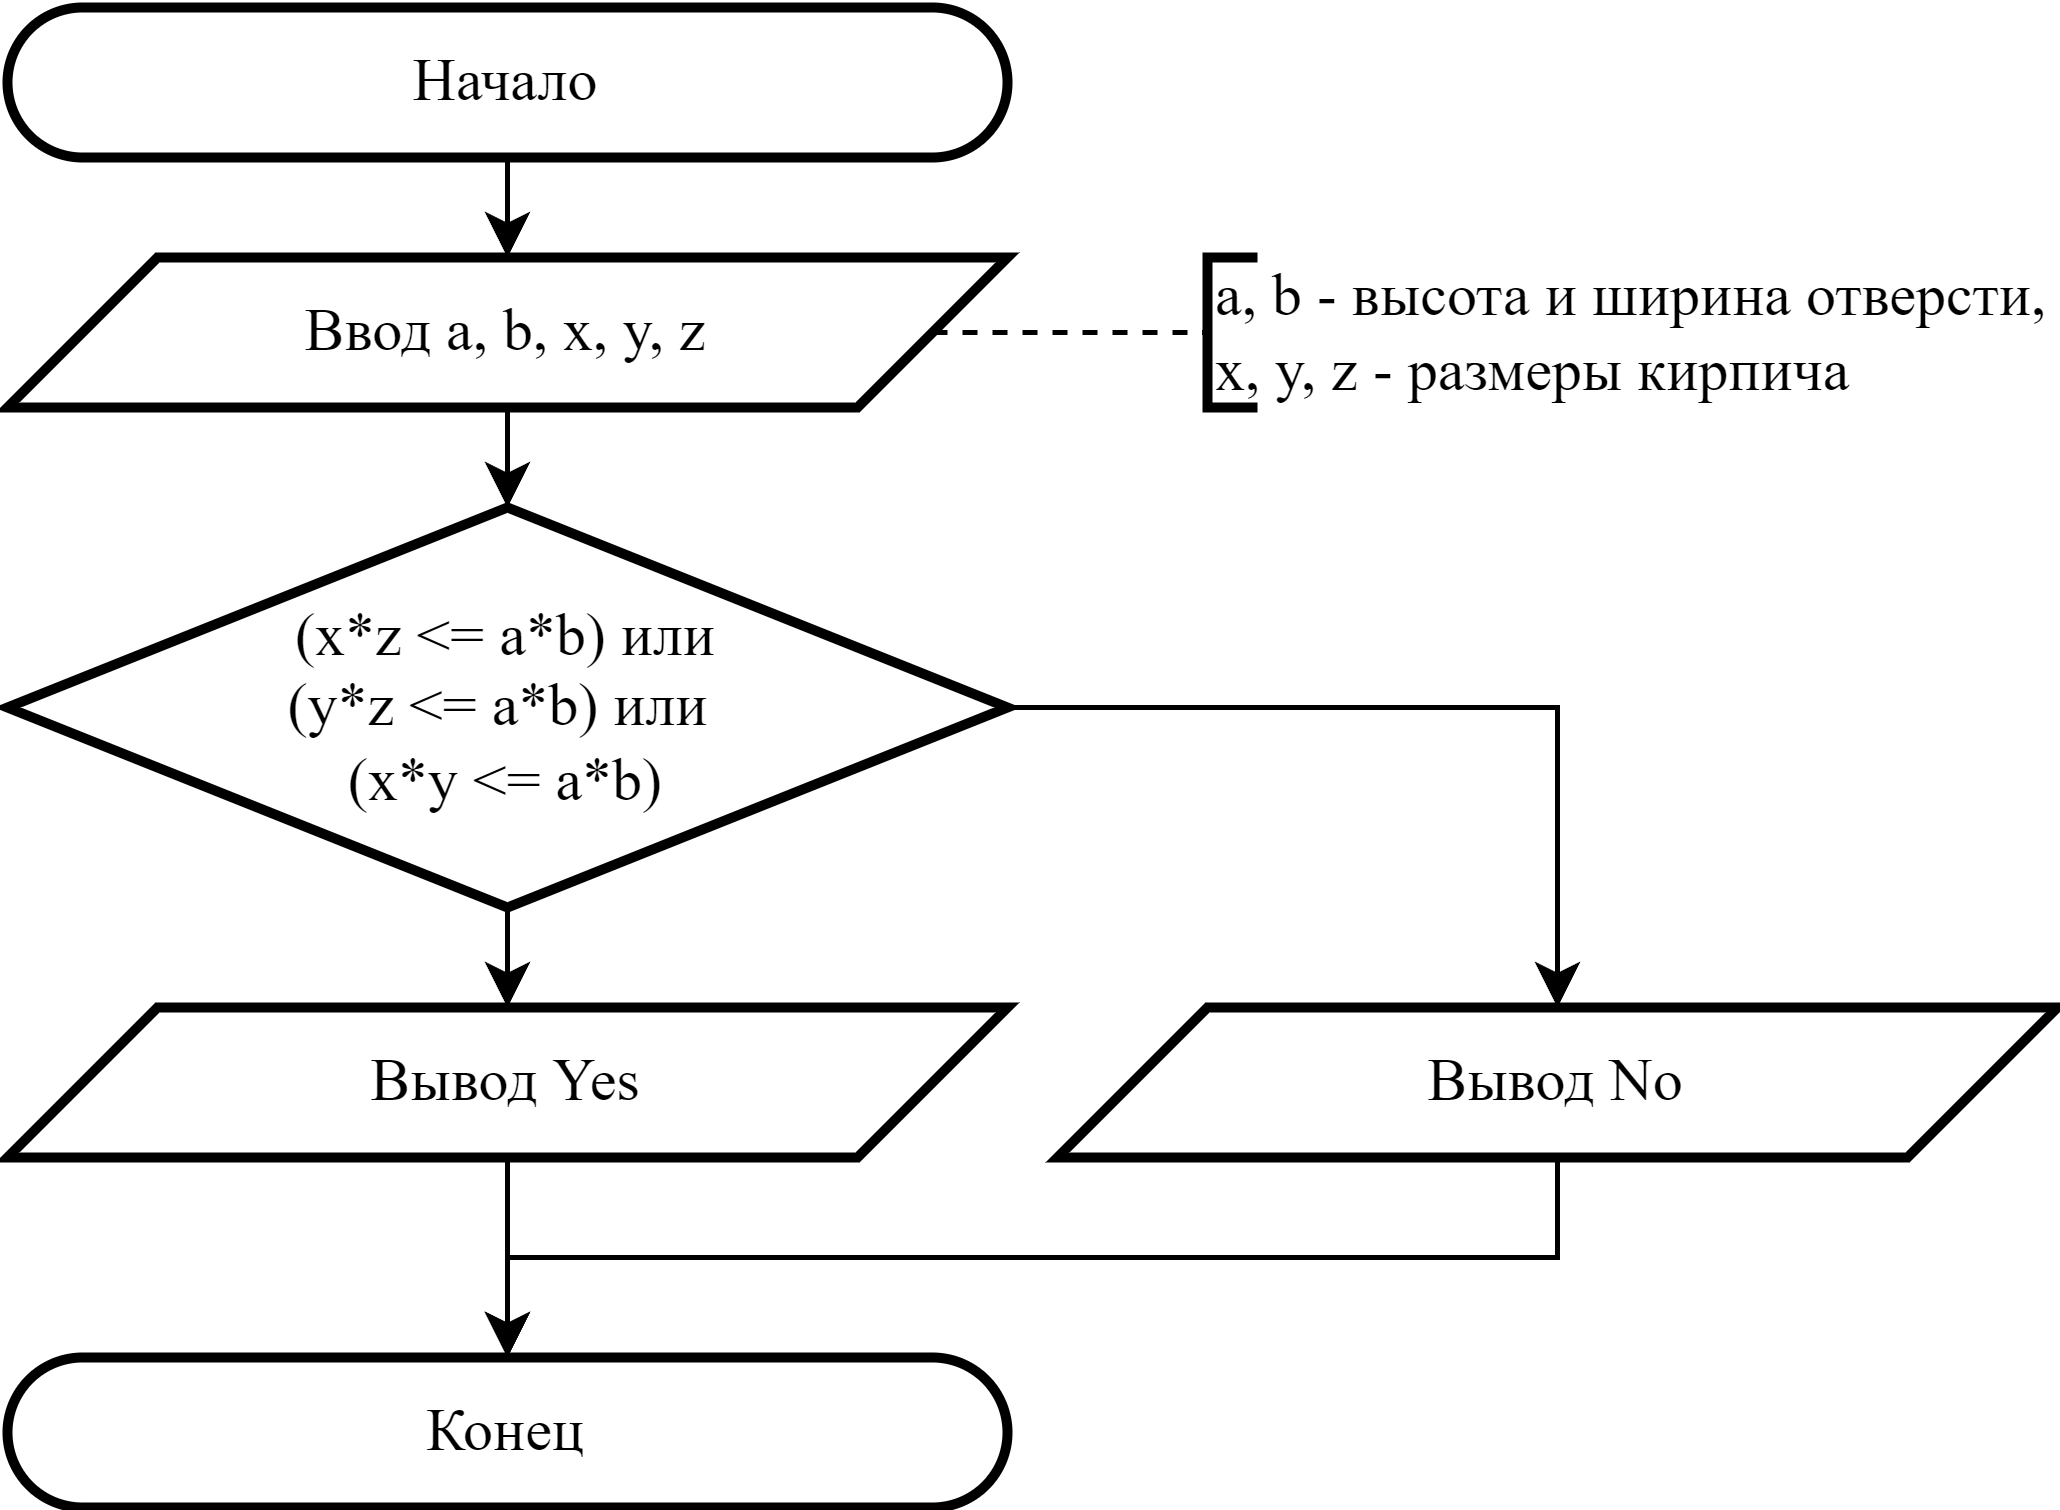
\includegraphics[width=0.75\textwidth]{img/5-scheme.png} % Укажите путь к изображению
	\caption{Схема алгоритма решения Задания 5.} % Подпись к изображению
\end{figure}
\begin{figure}
	\centering
	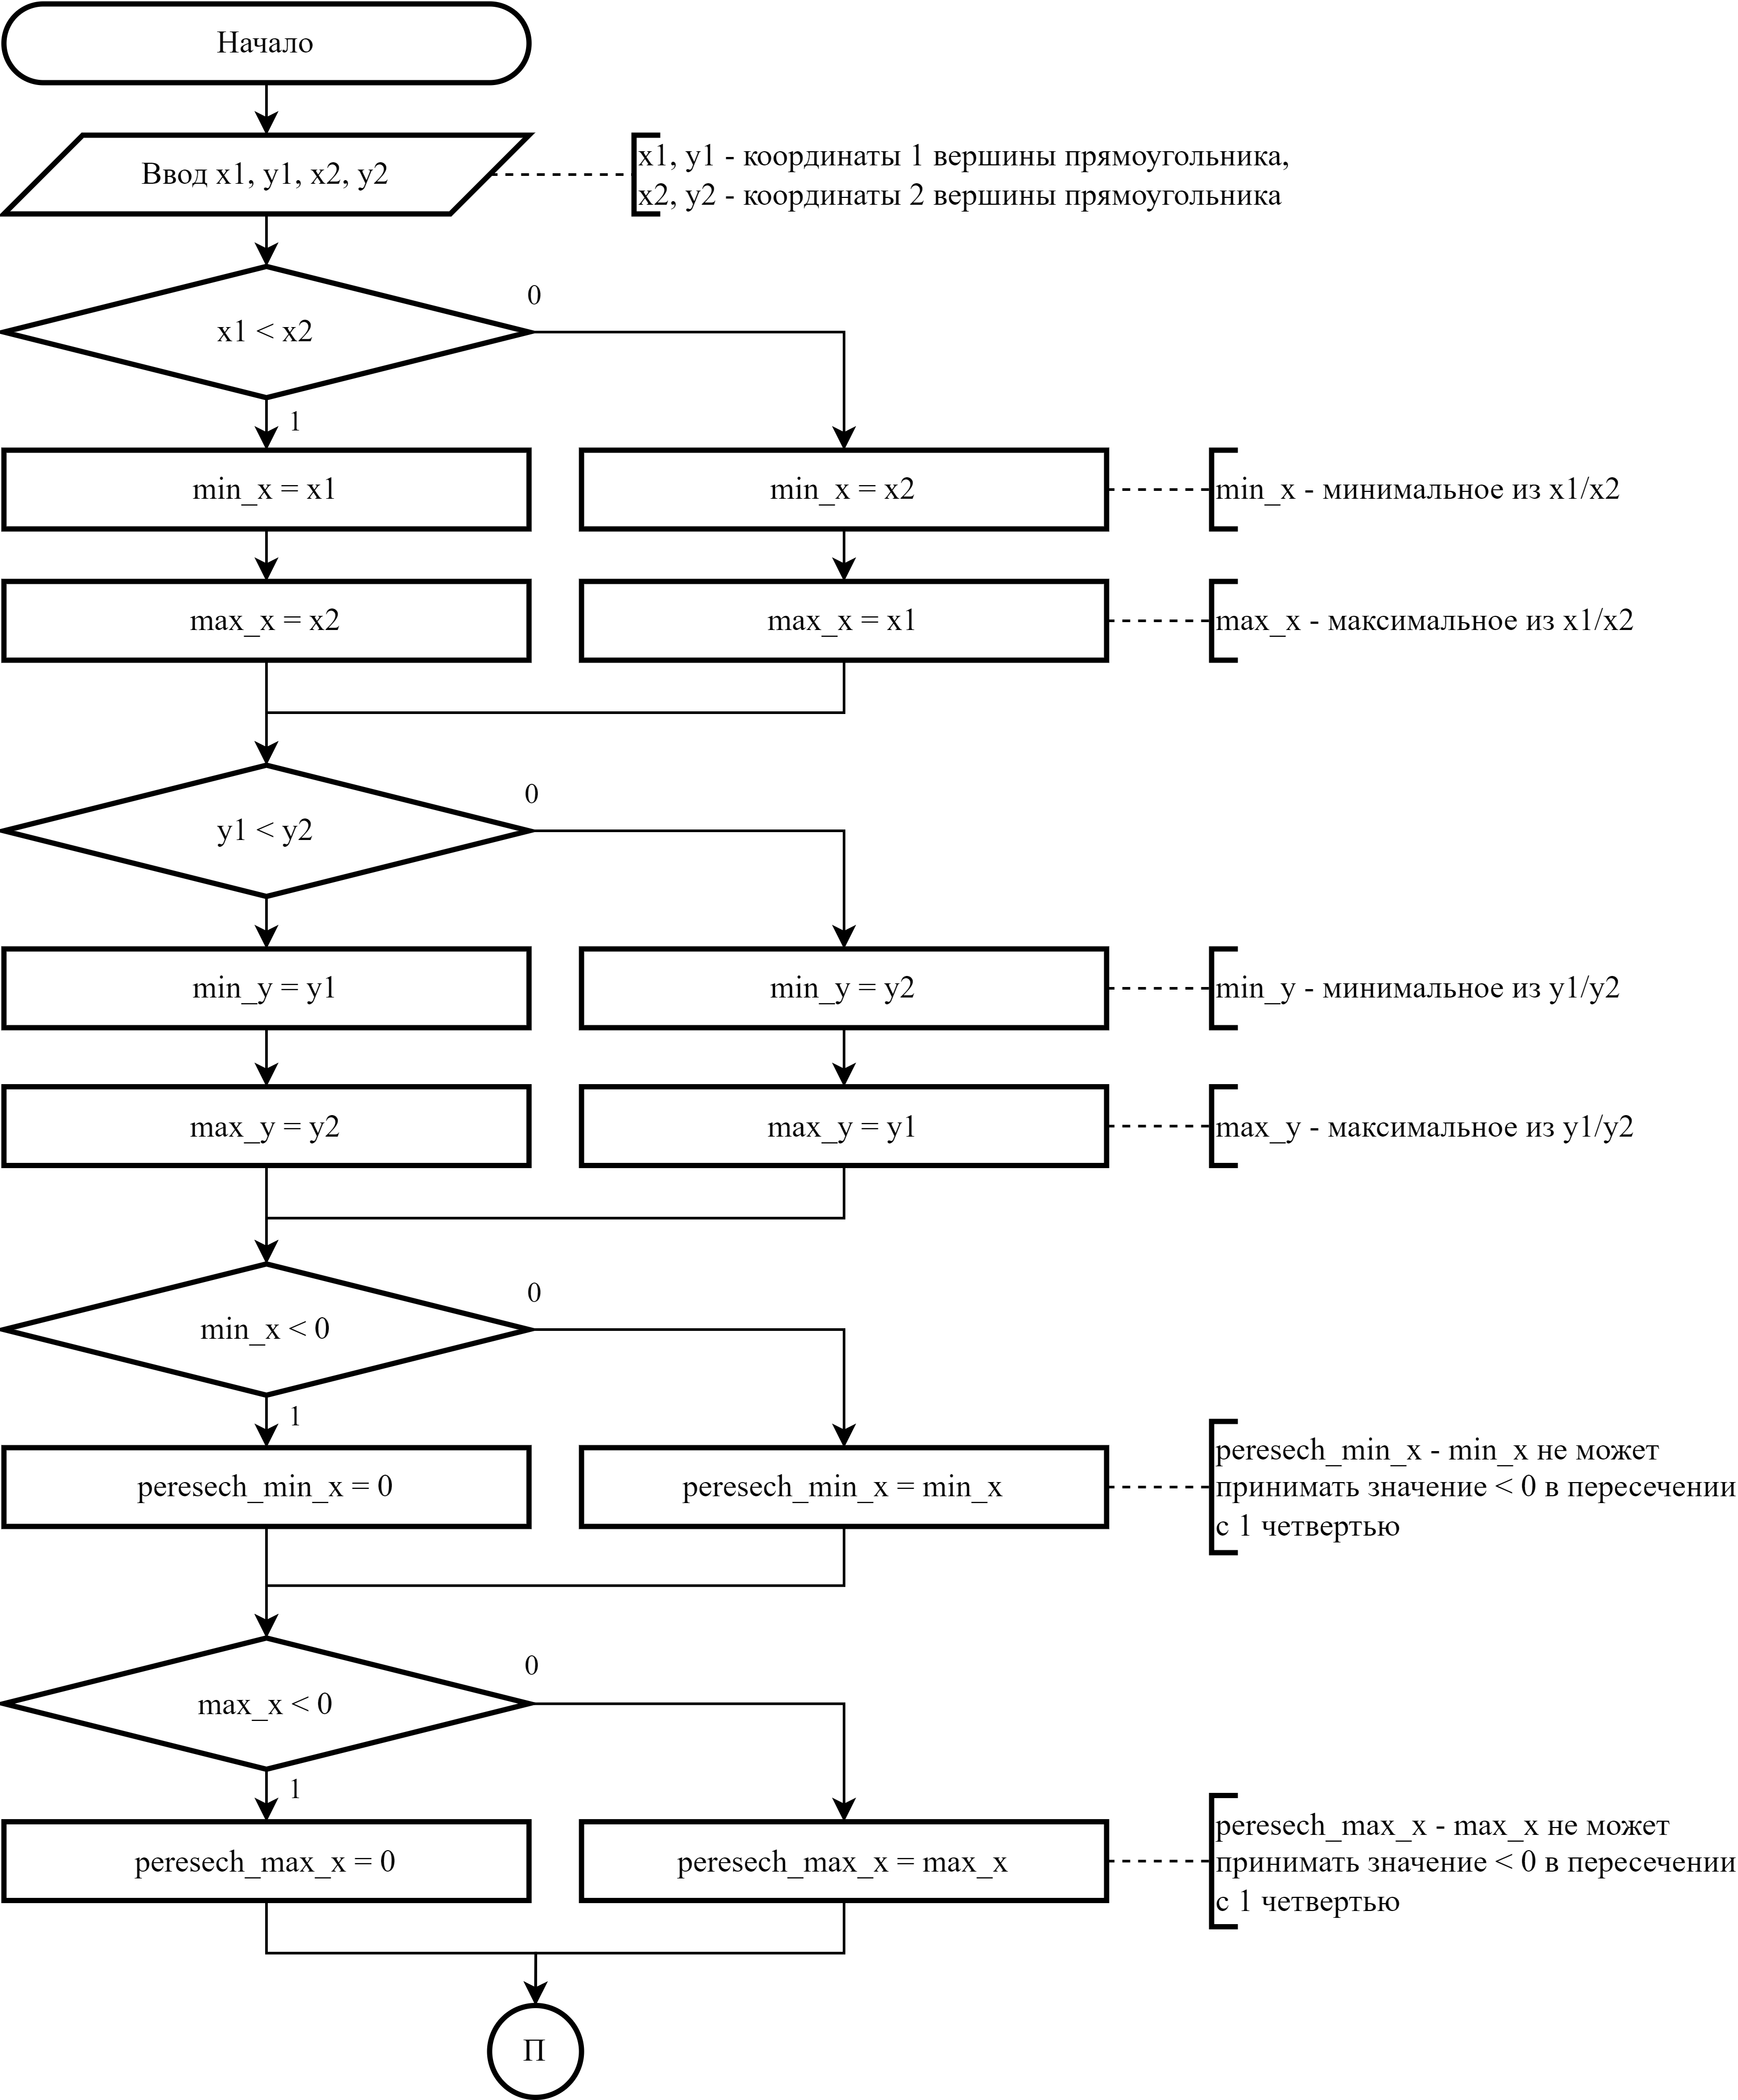
\includegraphics[height=0.9\textheight]{img/6-scheme-p1.png} % Укажите путь к изображению
\end{figure}
\begin{figure}
	\centering
	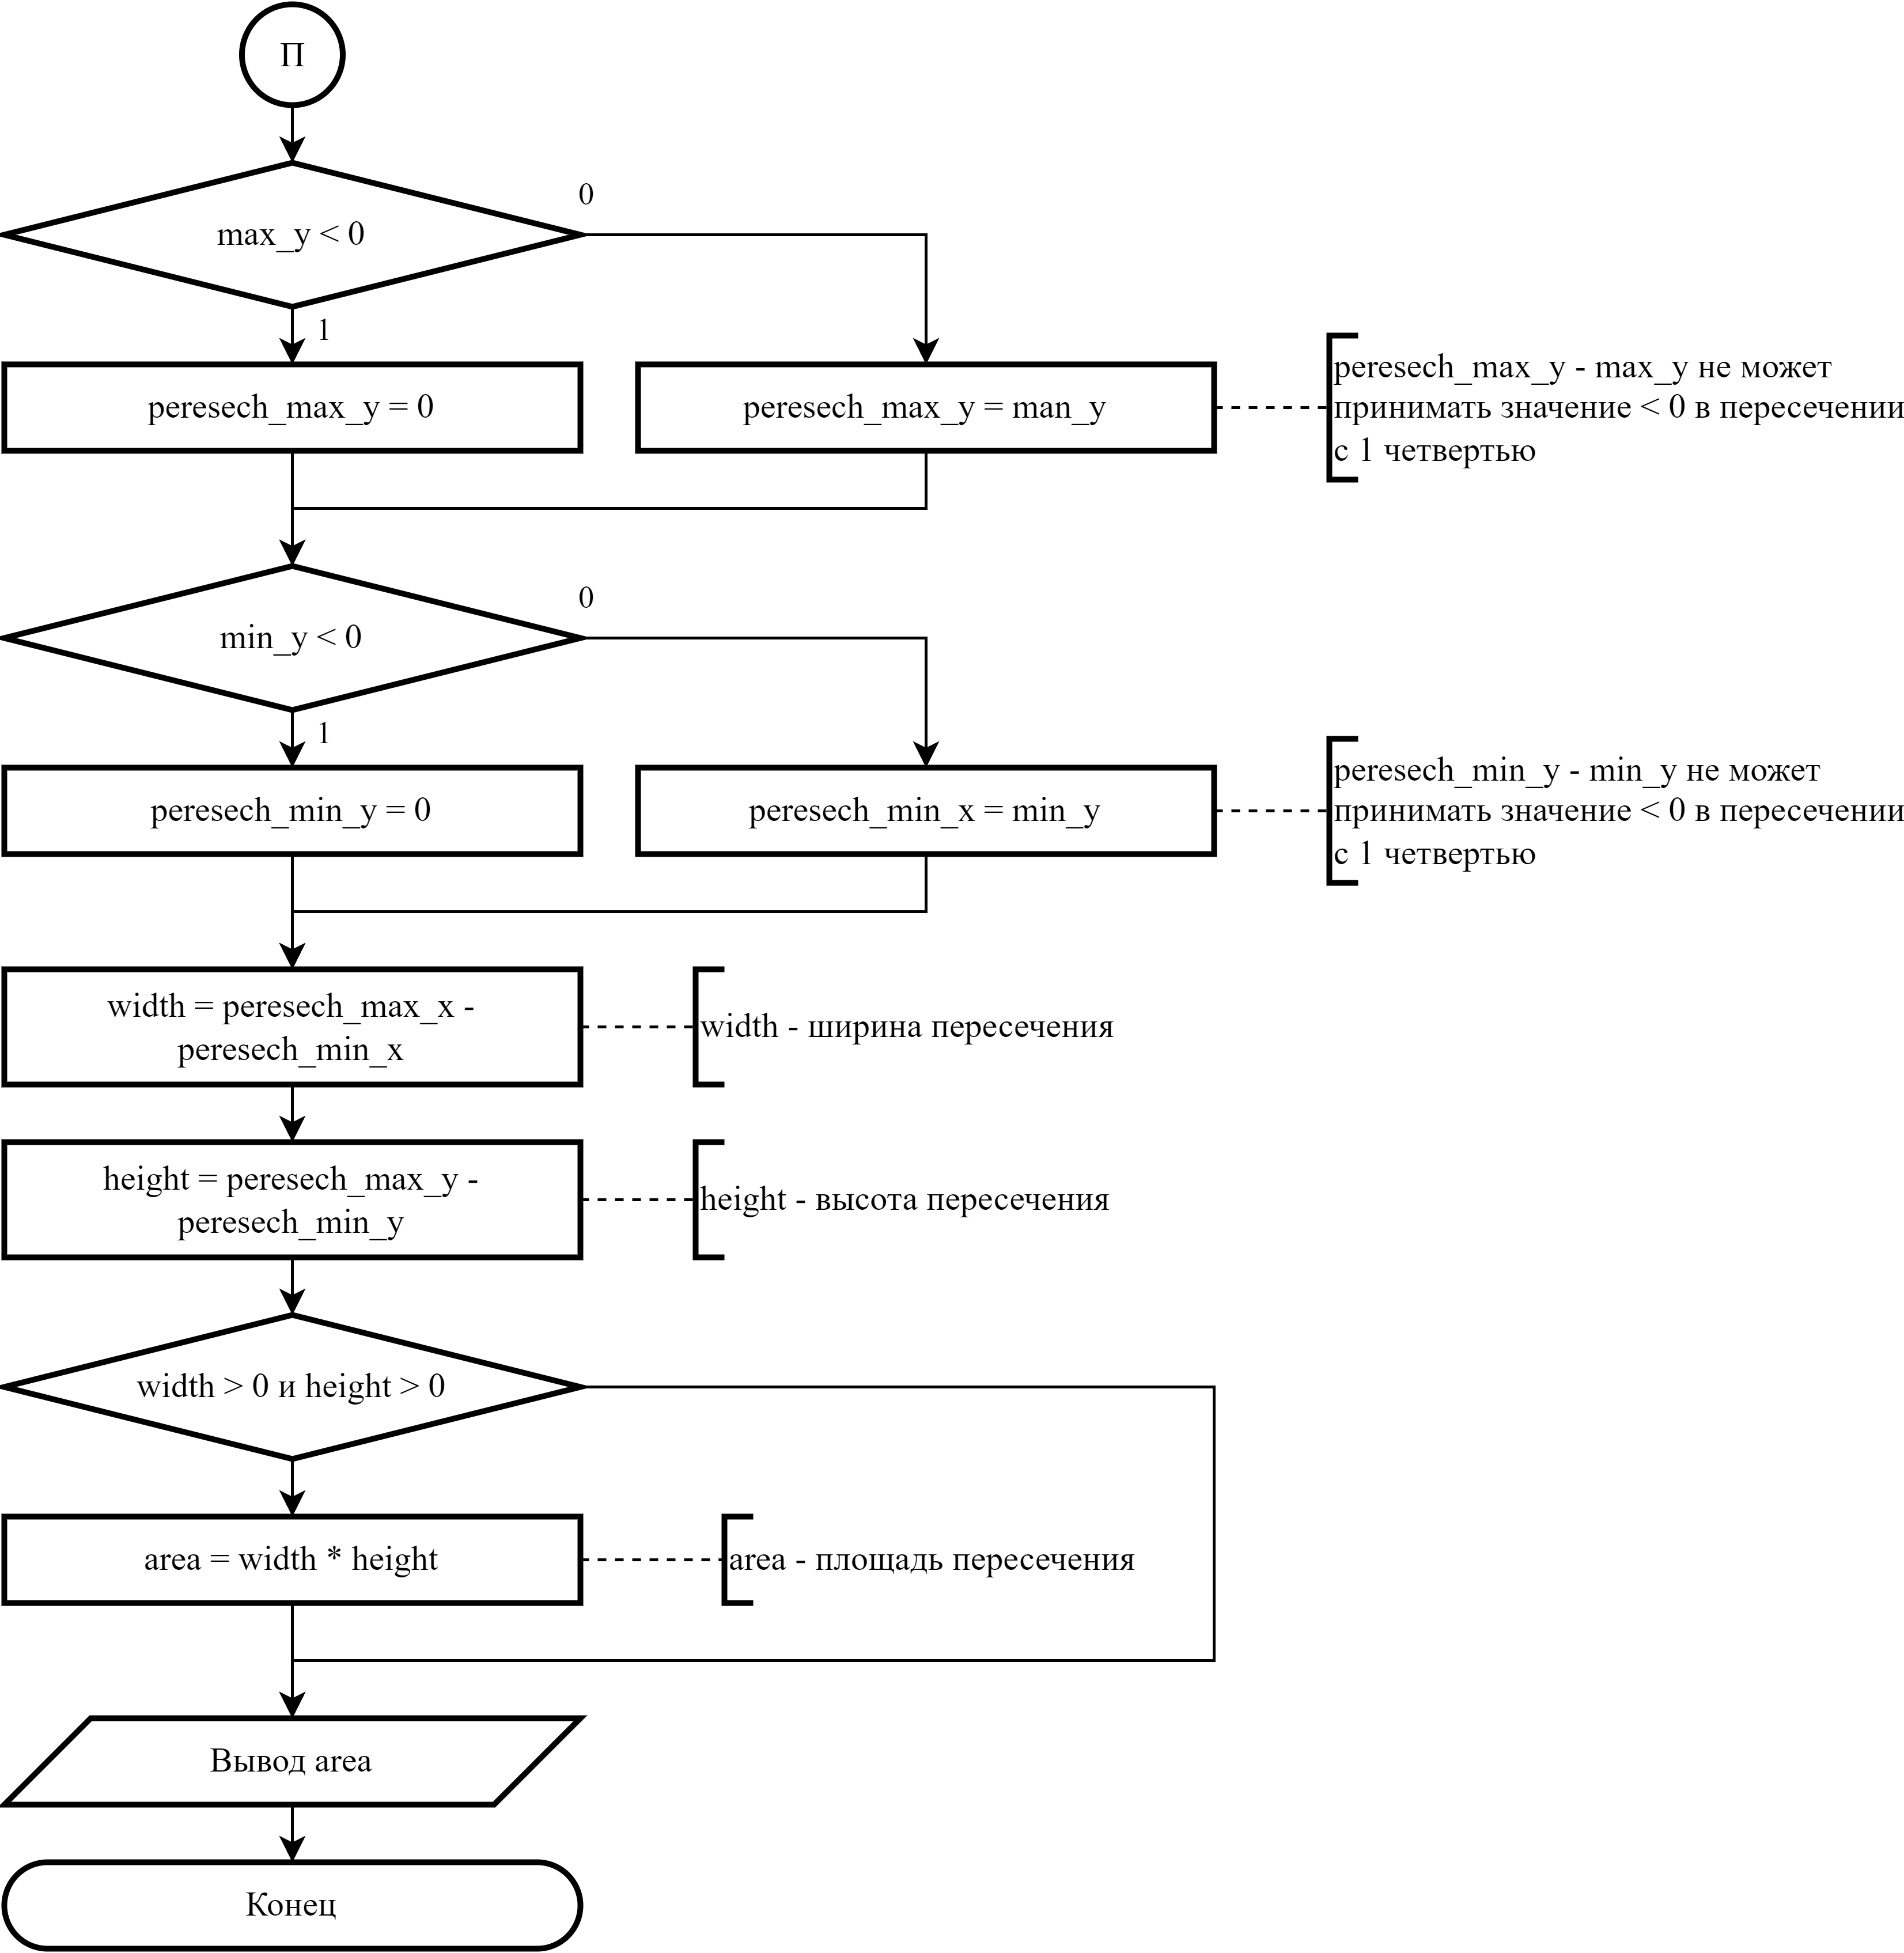
\includegraphics[width=\textwidth]{img/6-scheme-p2.png} % Укажите путь к изображению
	\caption{Схема алгоритма решения Задания 6.} % Подпись к изображению
\end{figure}
\begin{figure}
	\centering
	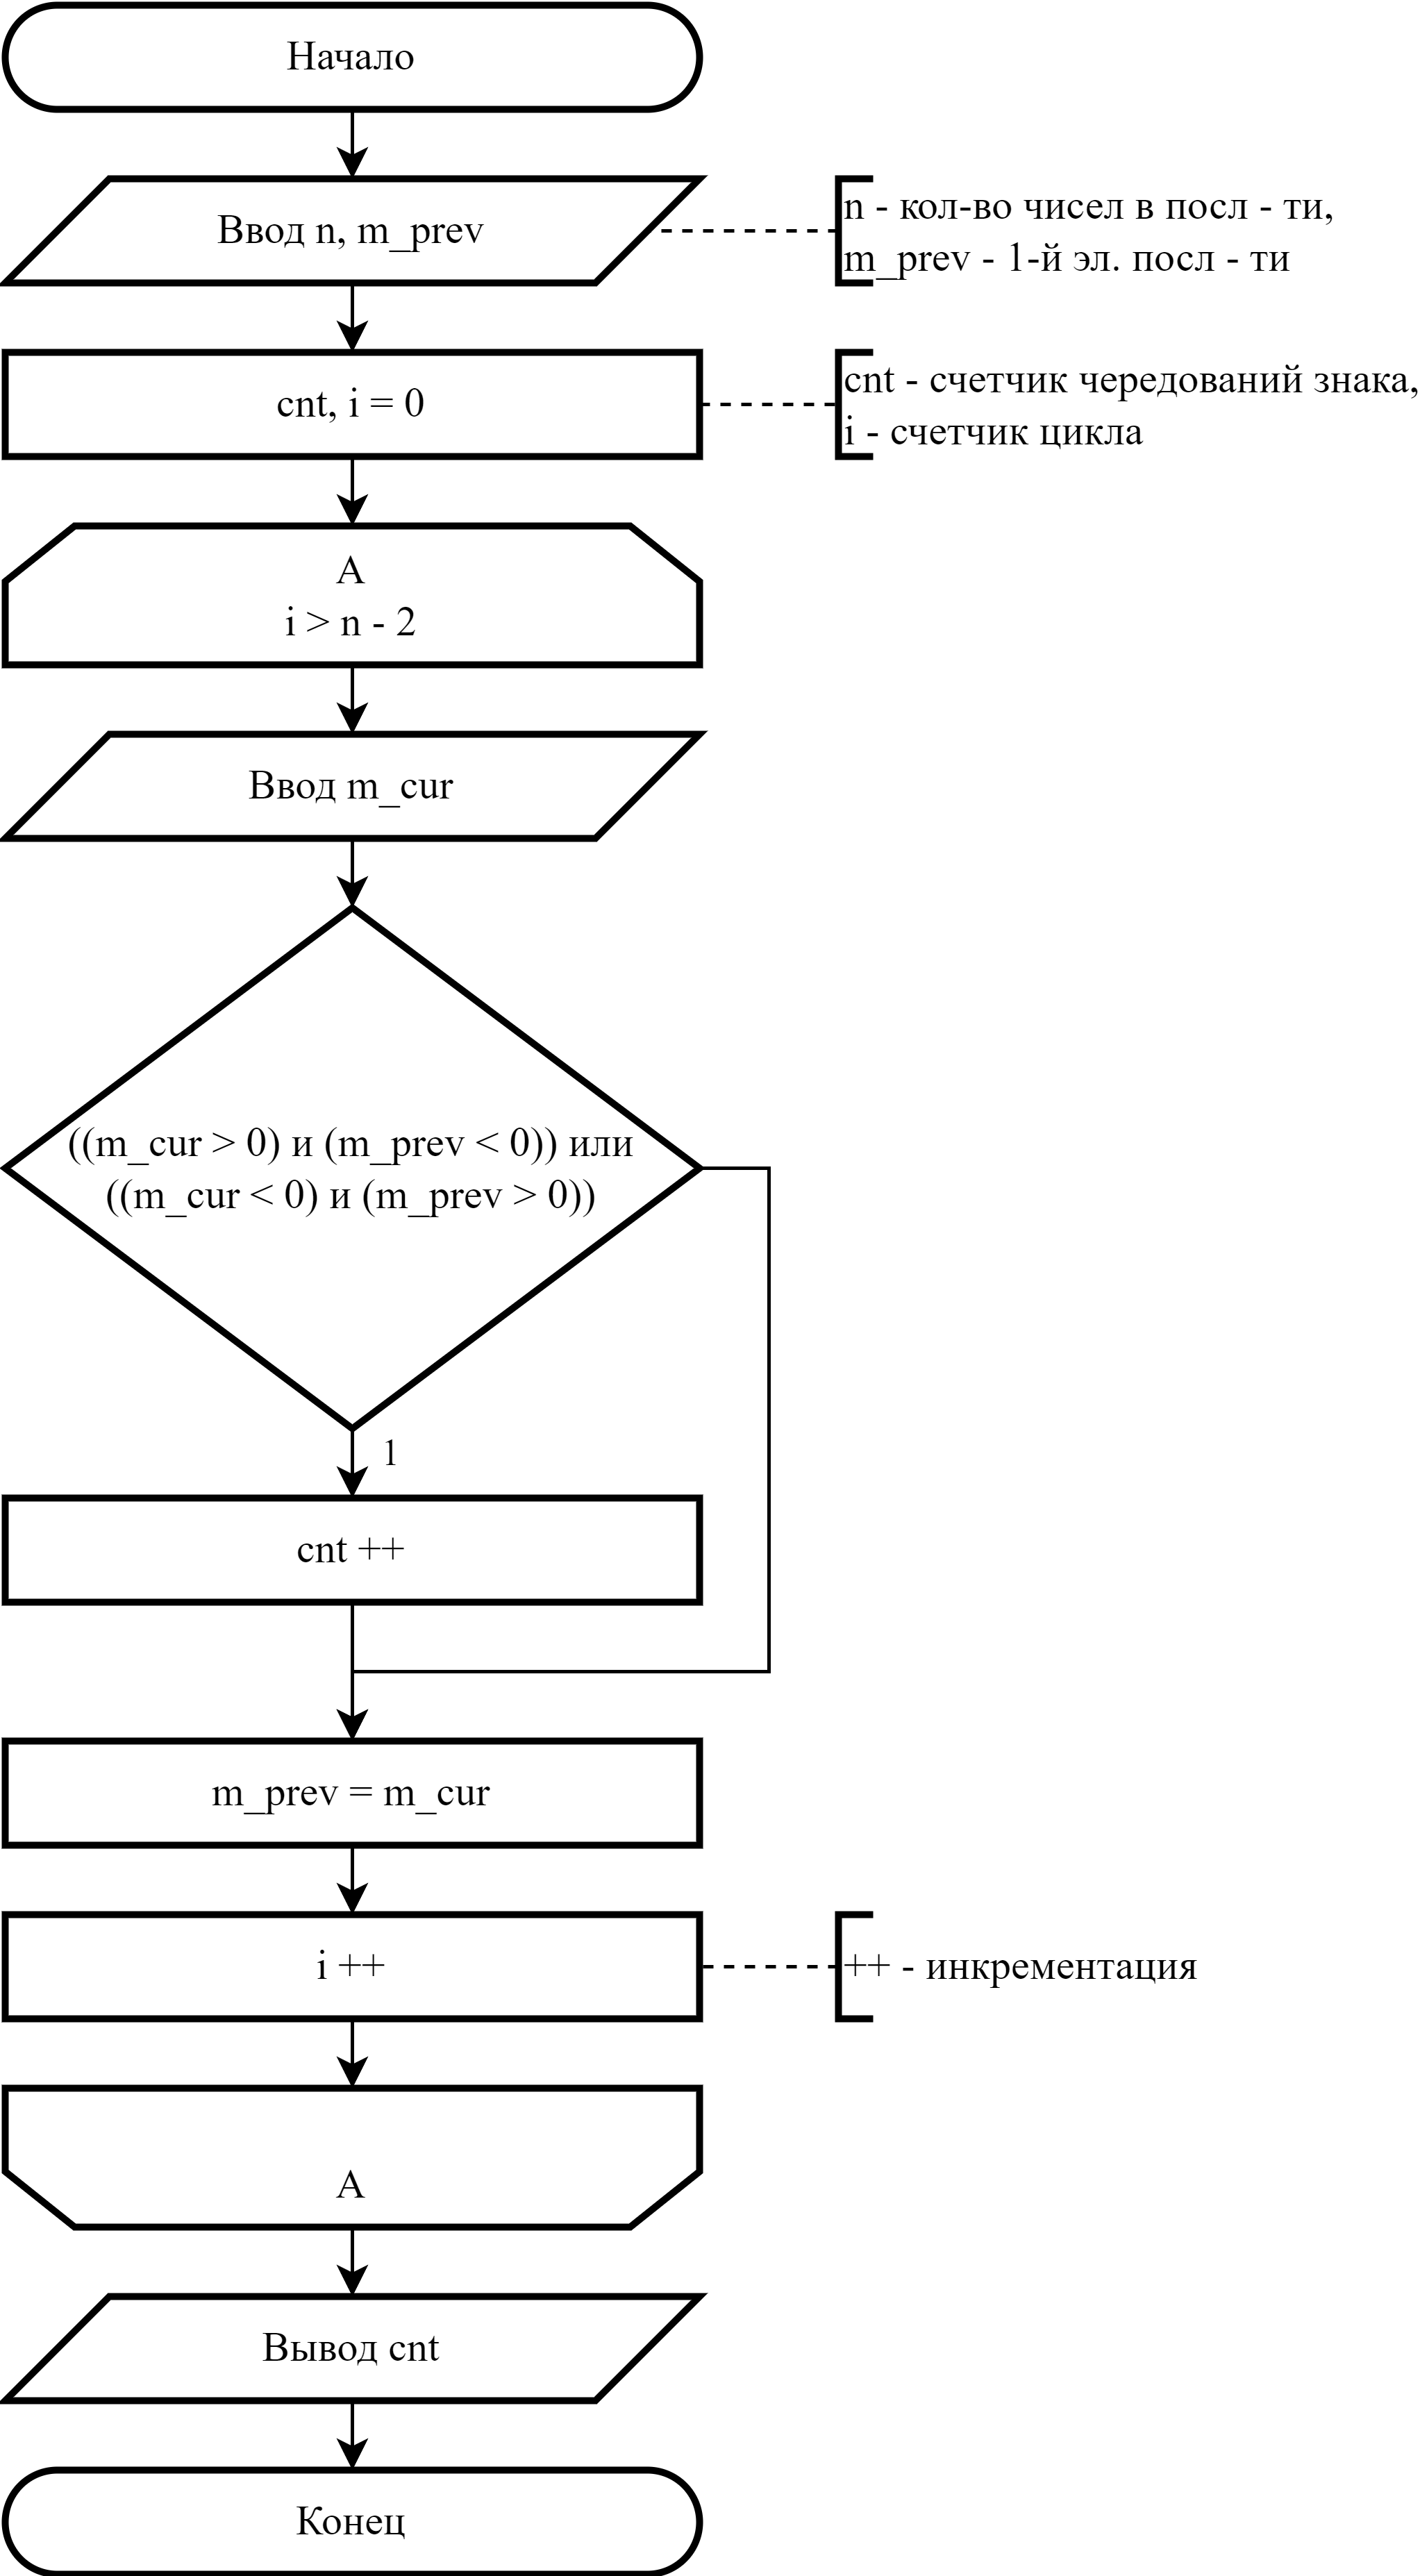
\includegraphics[height=0.8\textheight]{img/7-scheme.png} % Укажите путь к изображению
	\caption{Схема алгоритма решения Задания 7.} % Подпись к изображению
\end{figure}
\begin{figure}
	\centering
	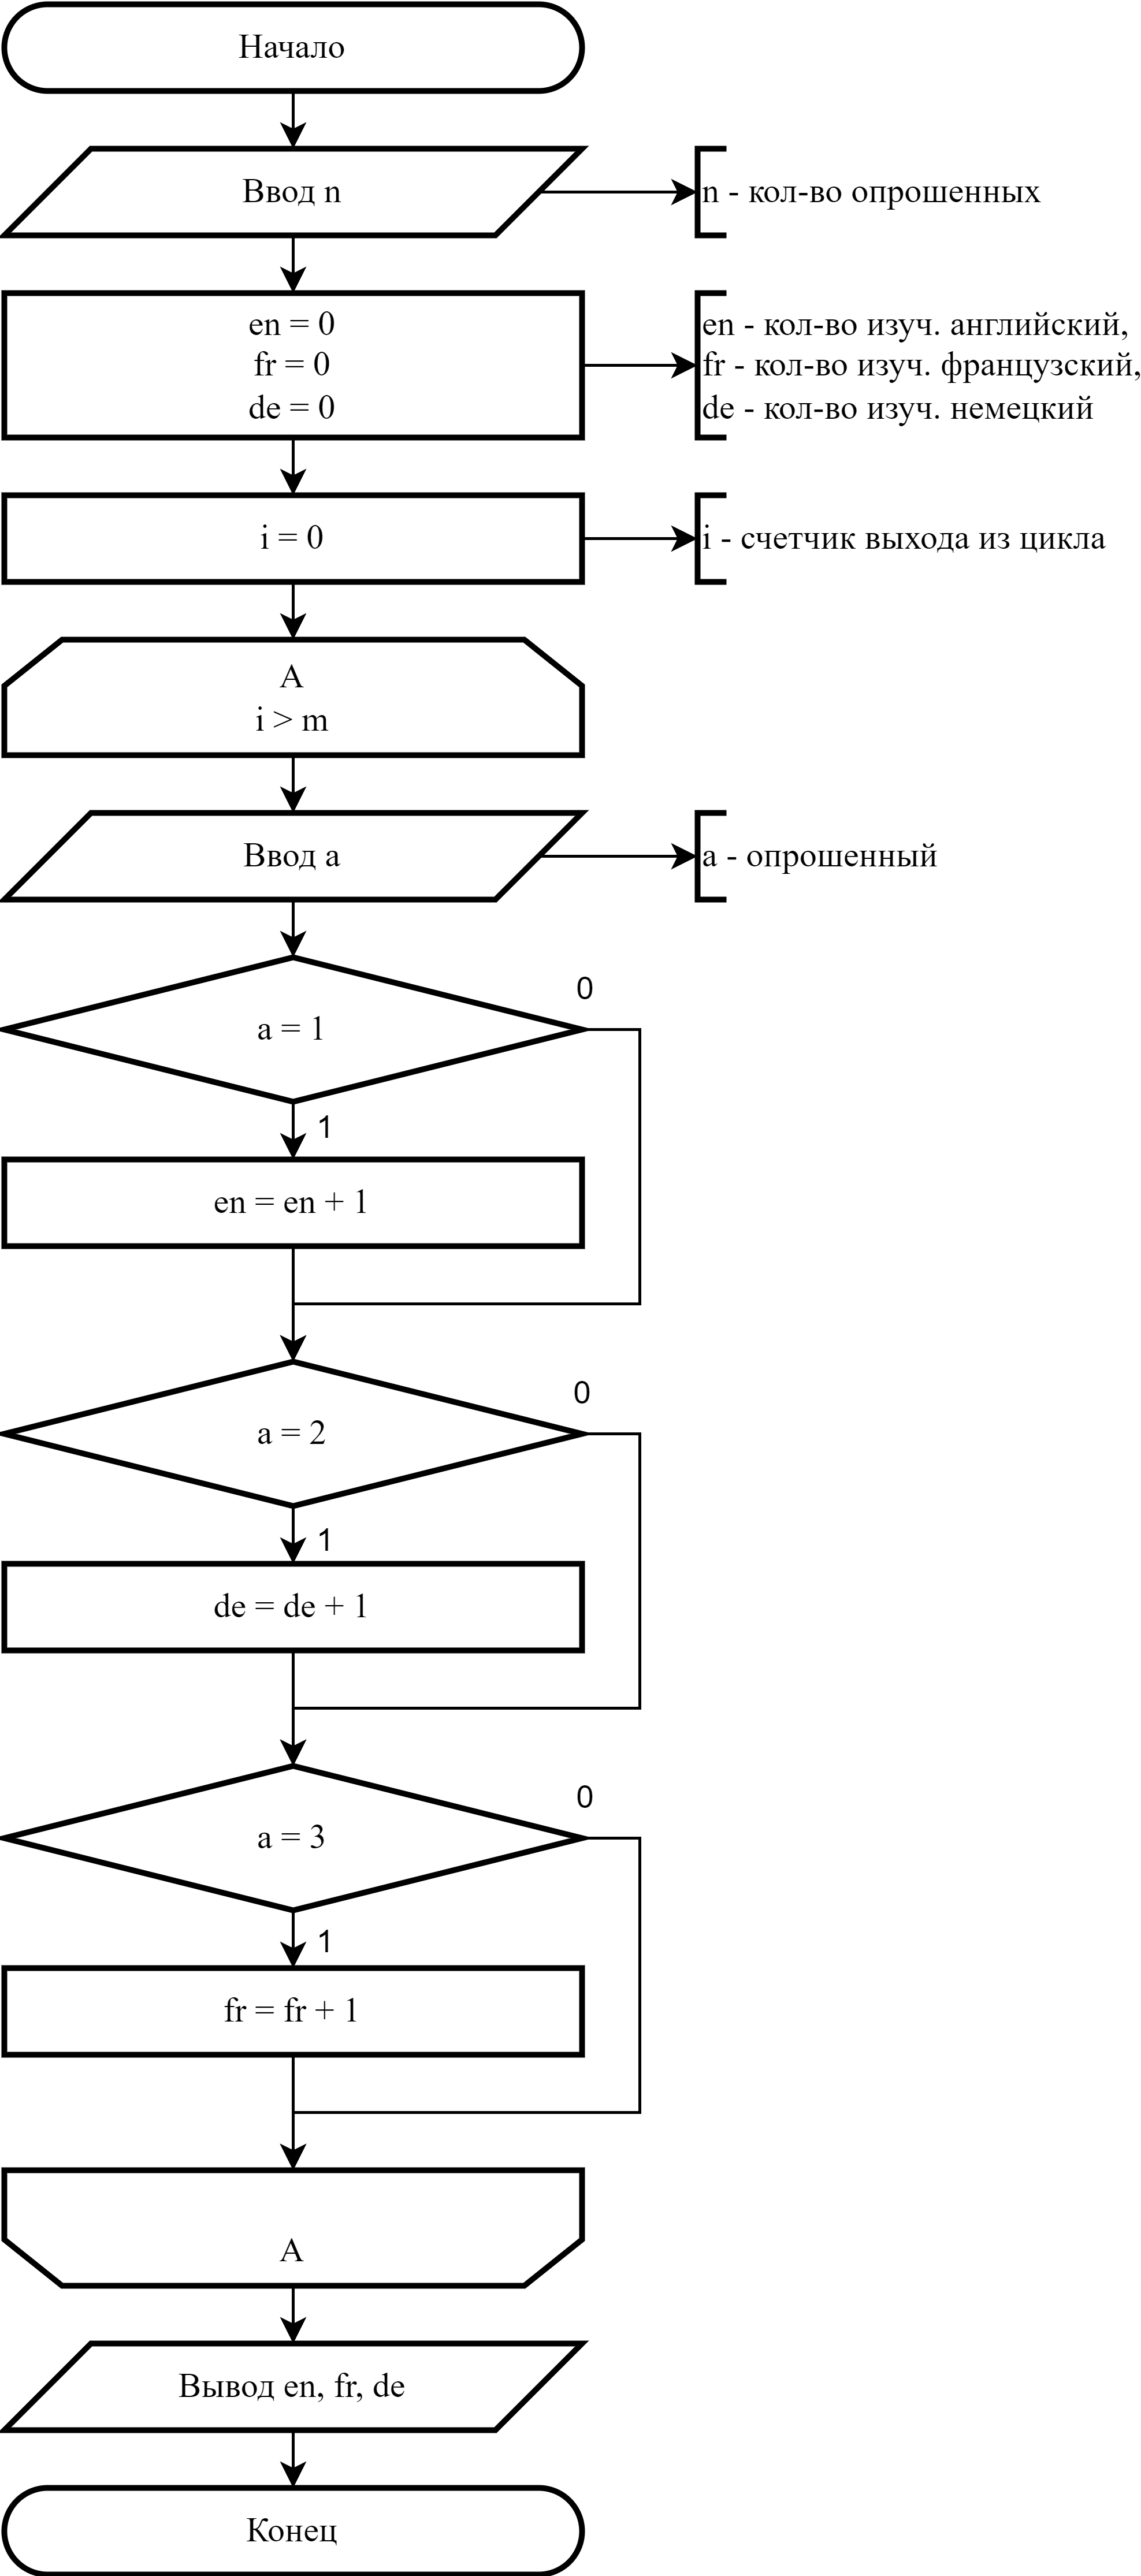
\includegraphics[height=0.9\textheight]{img/8-scheme.png} % Укажите путь к изображению
	\caption{Схема алгоритма решения Задания 8.} % Подпись к изображению
\end{figure}
\begin{figure}
	\centering
	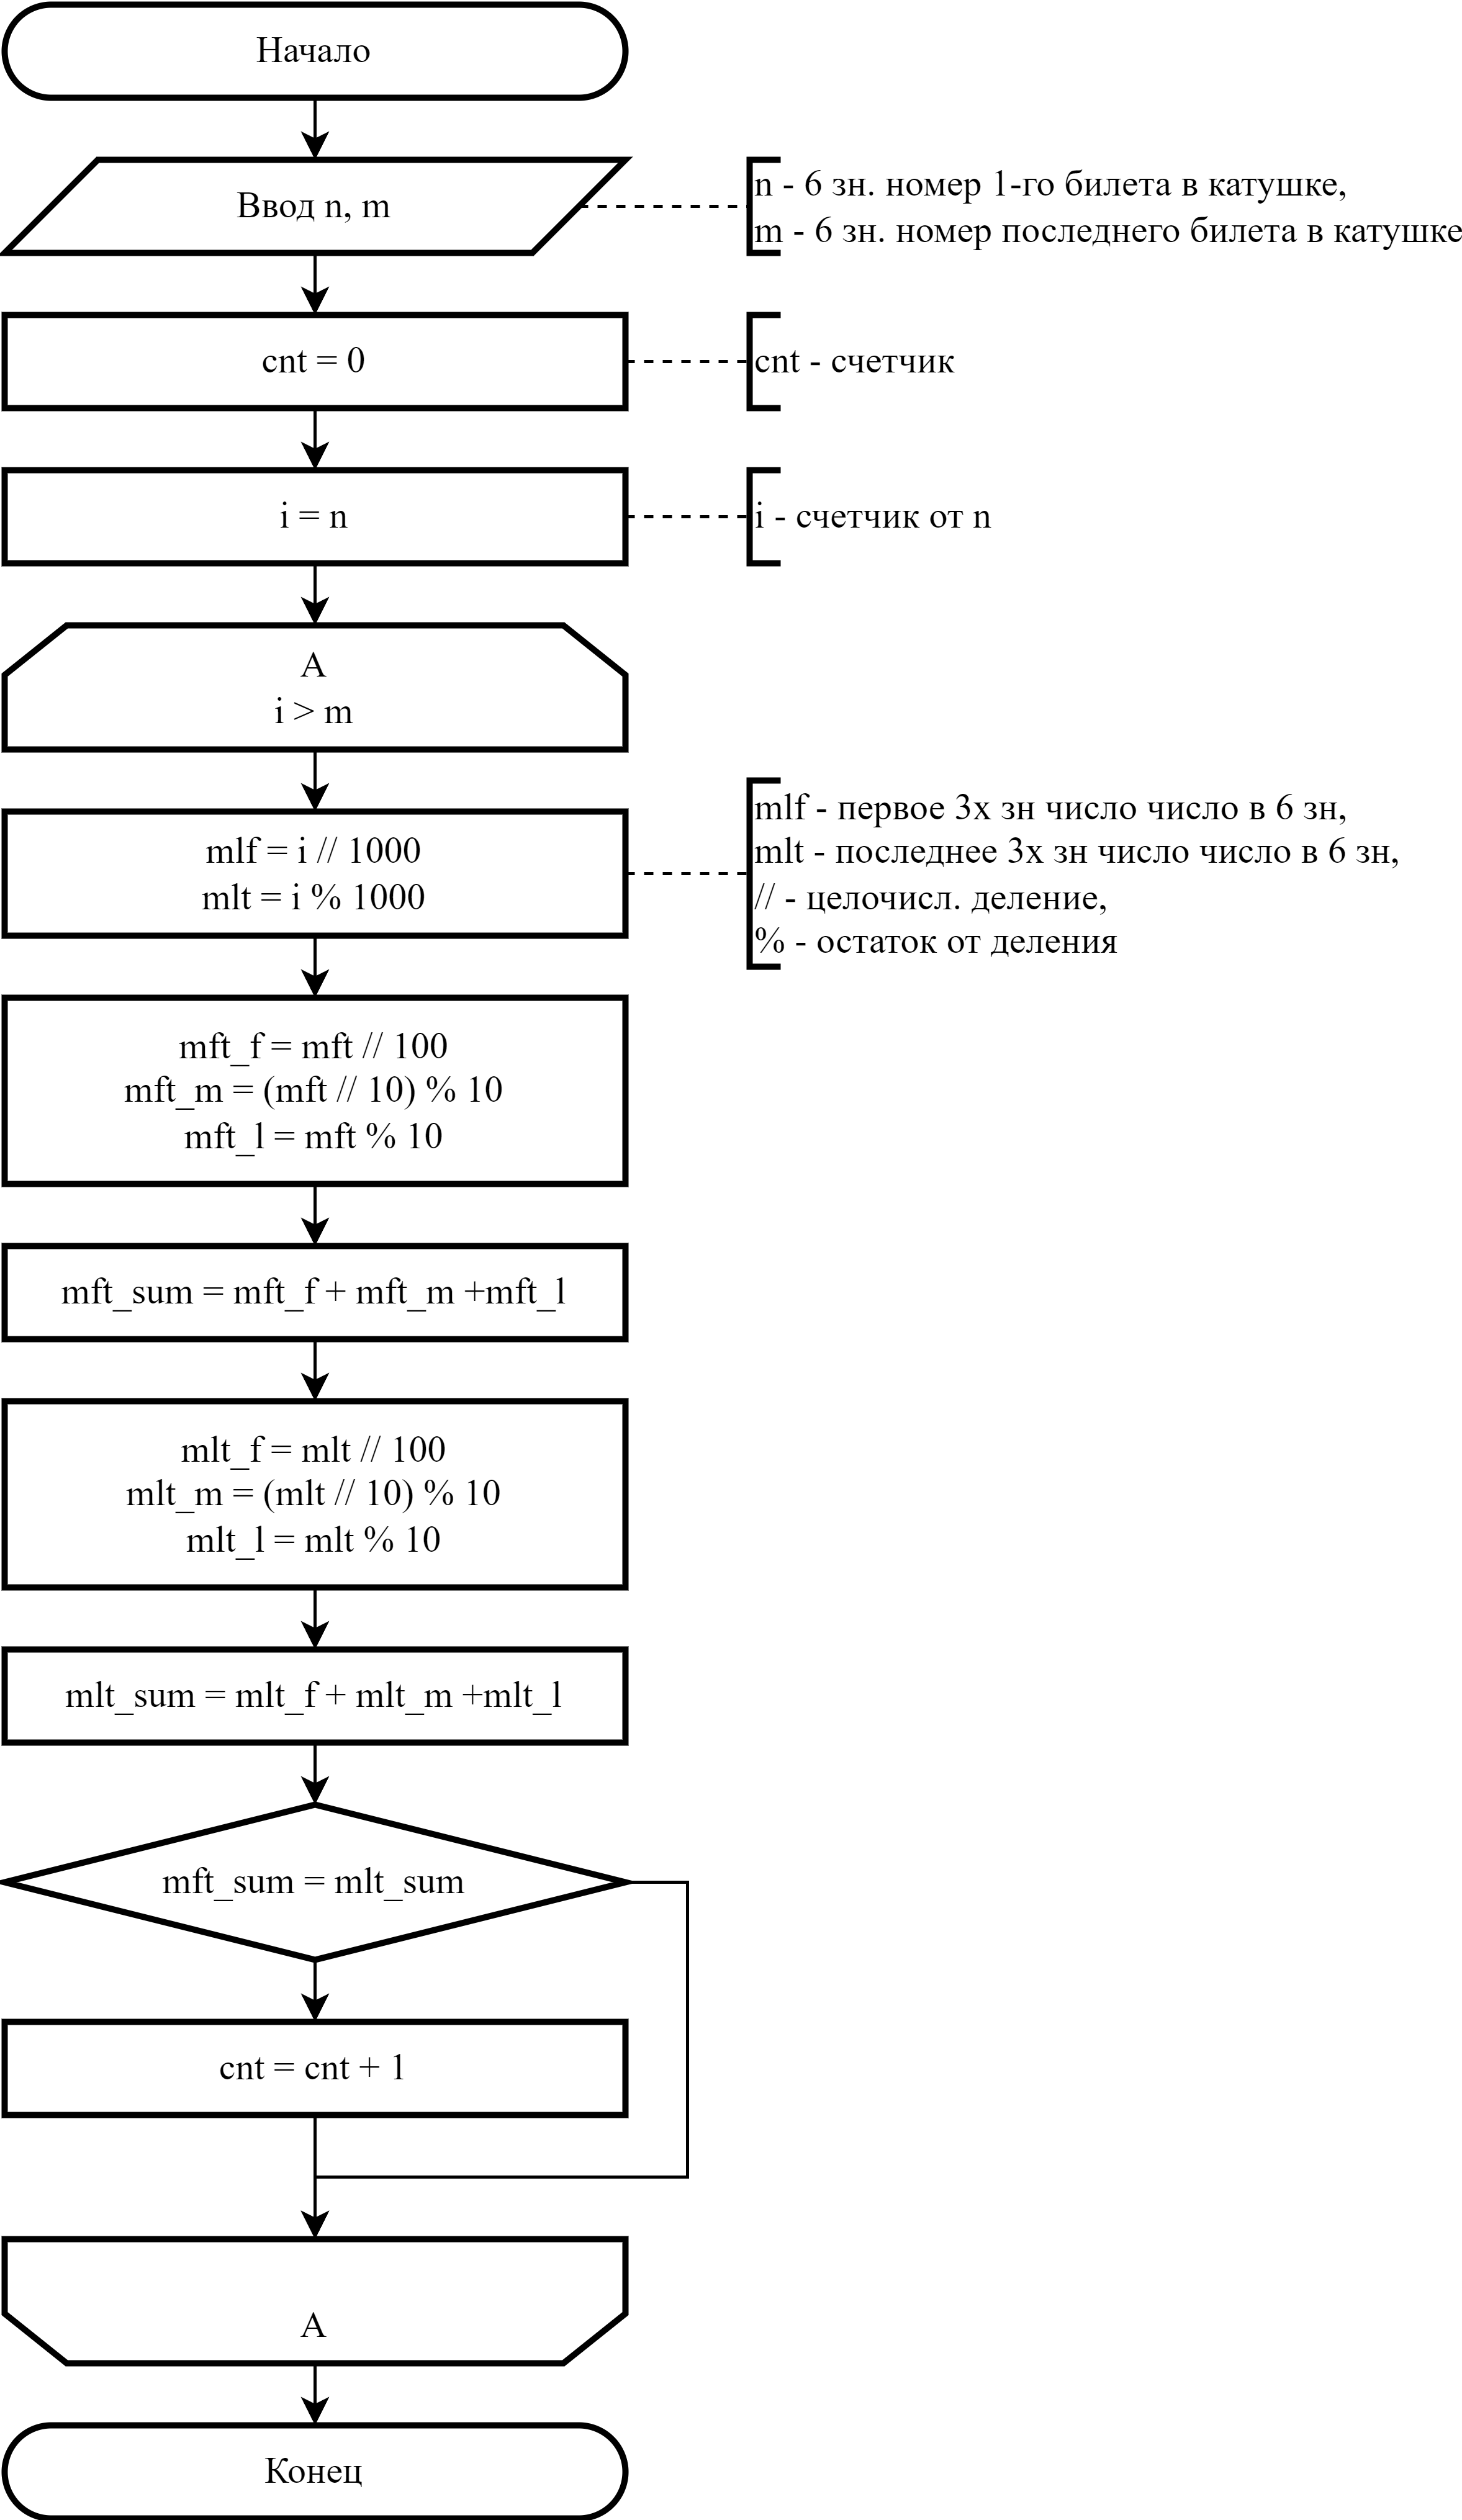
\includegraphics[height=0.9\textheight]{img/9-scheme.png} % Укажите путь к изображению
	\caption{Схема алгоритма решения Задания 9.} % Подпись к изображению
\end{figure}
\begin{figure}
	\centering
	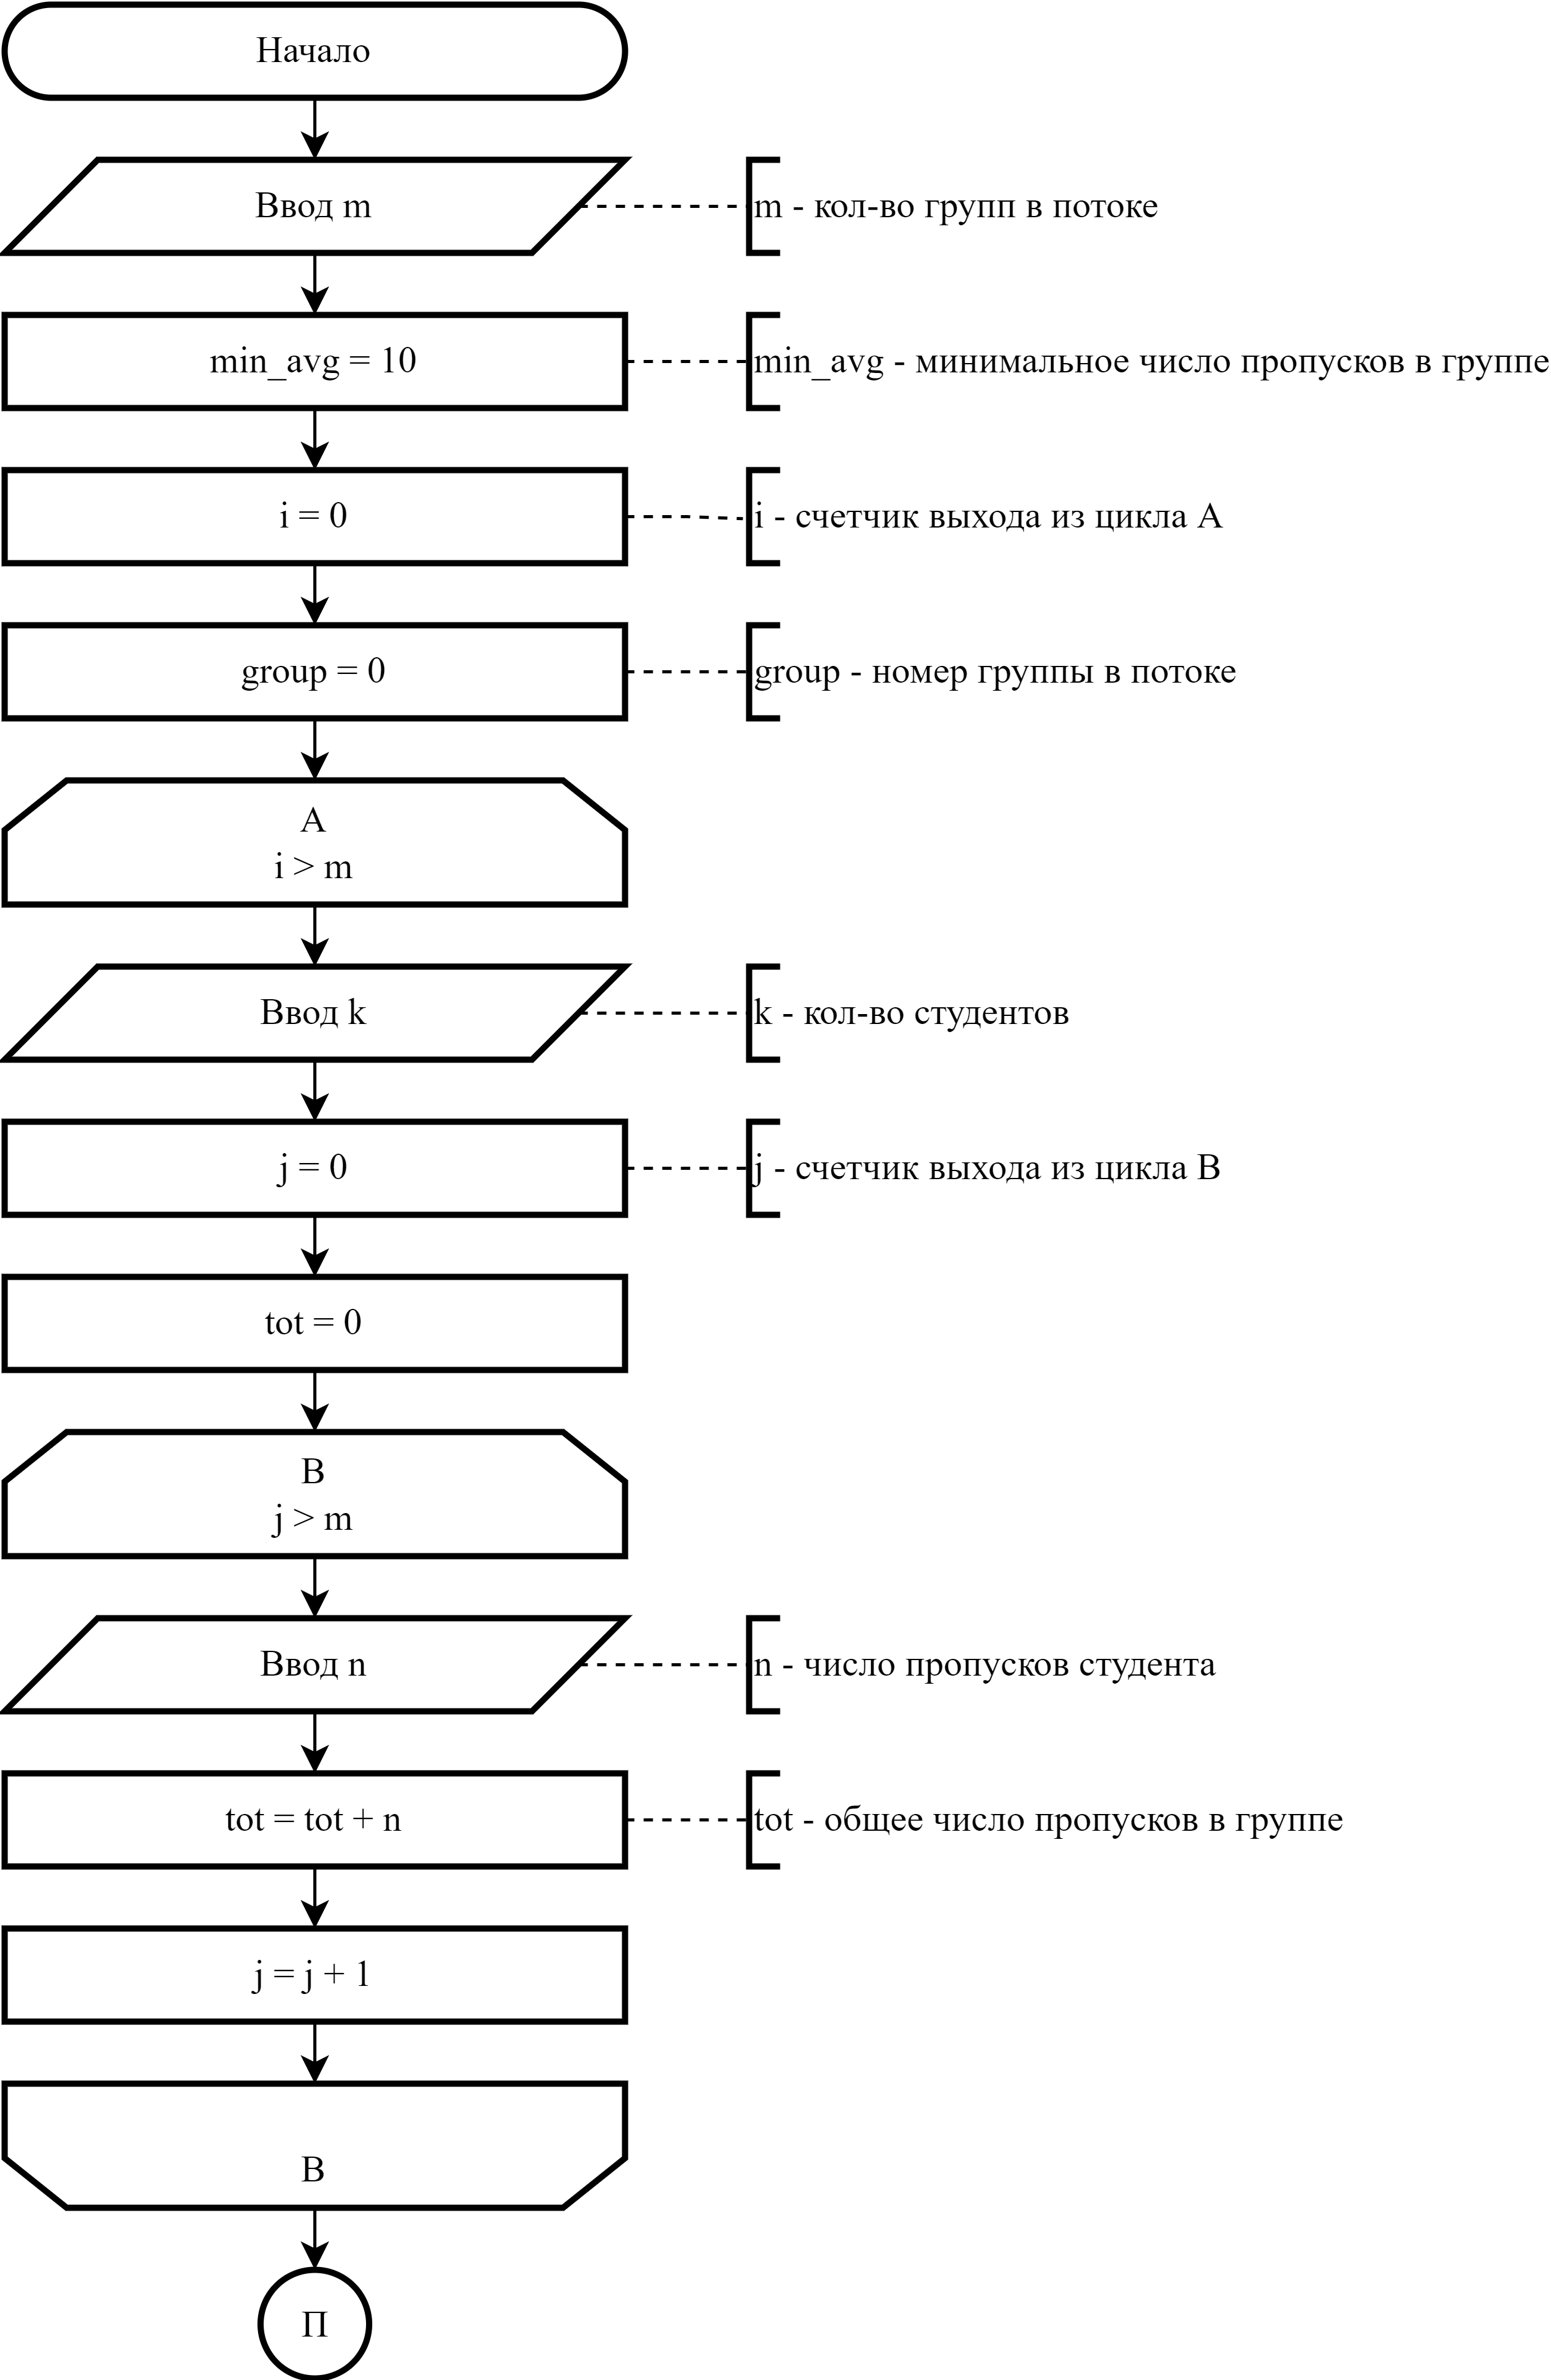
\includegraphics[height=\textheight]{img/10-scheme-p1.png} % Укажите путь к изображению
\end{figure}
\begin{figure}
	\centering
	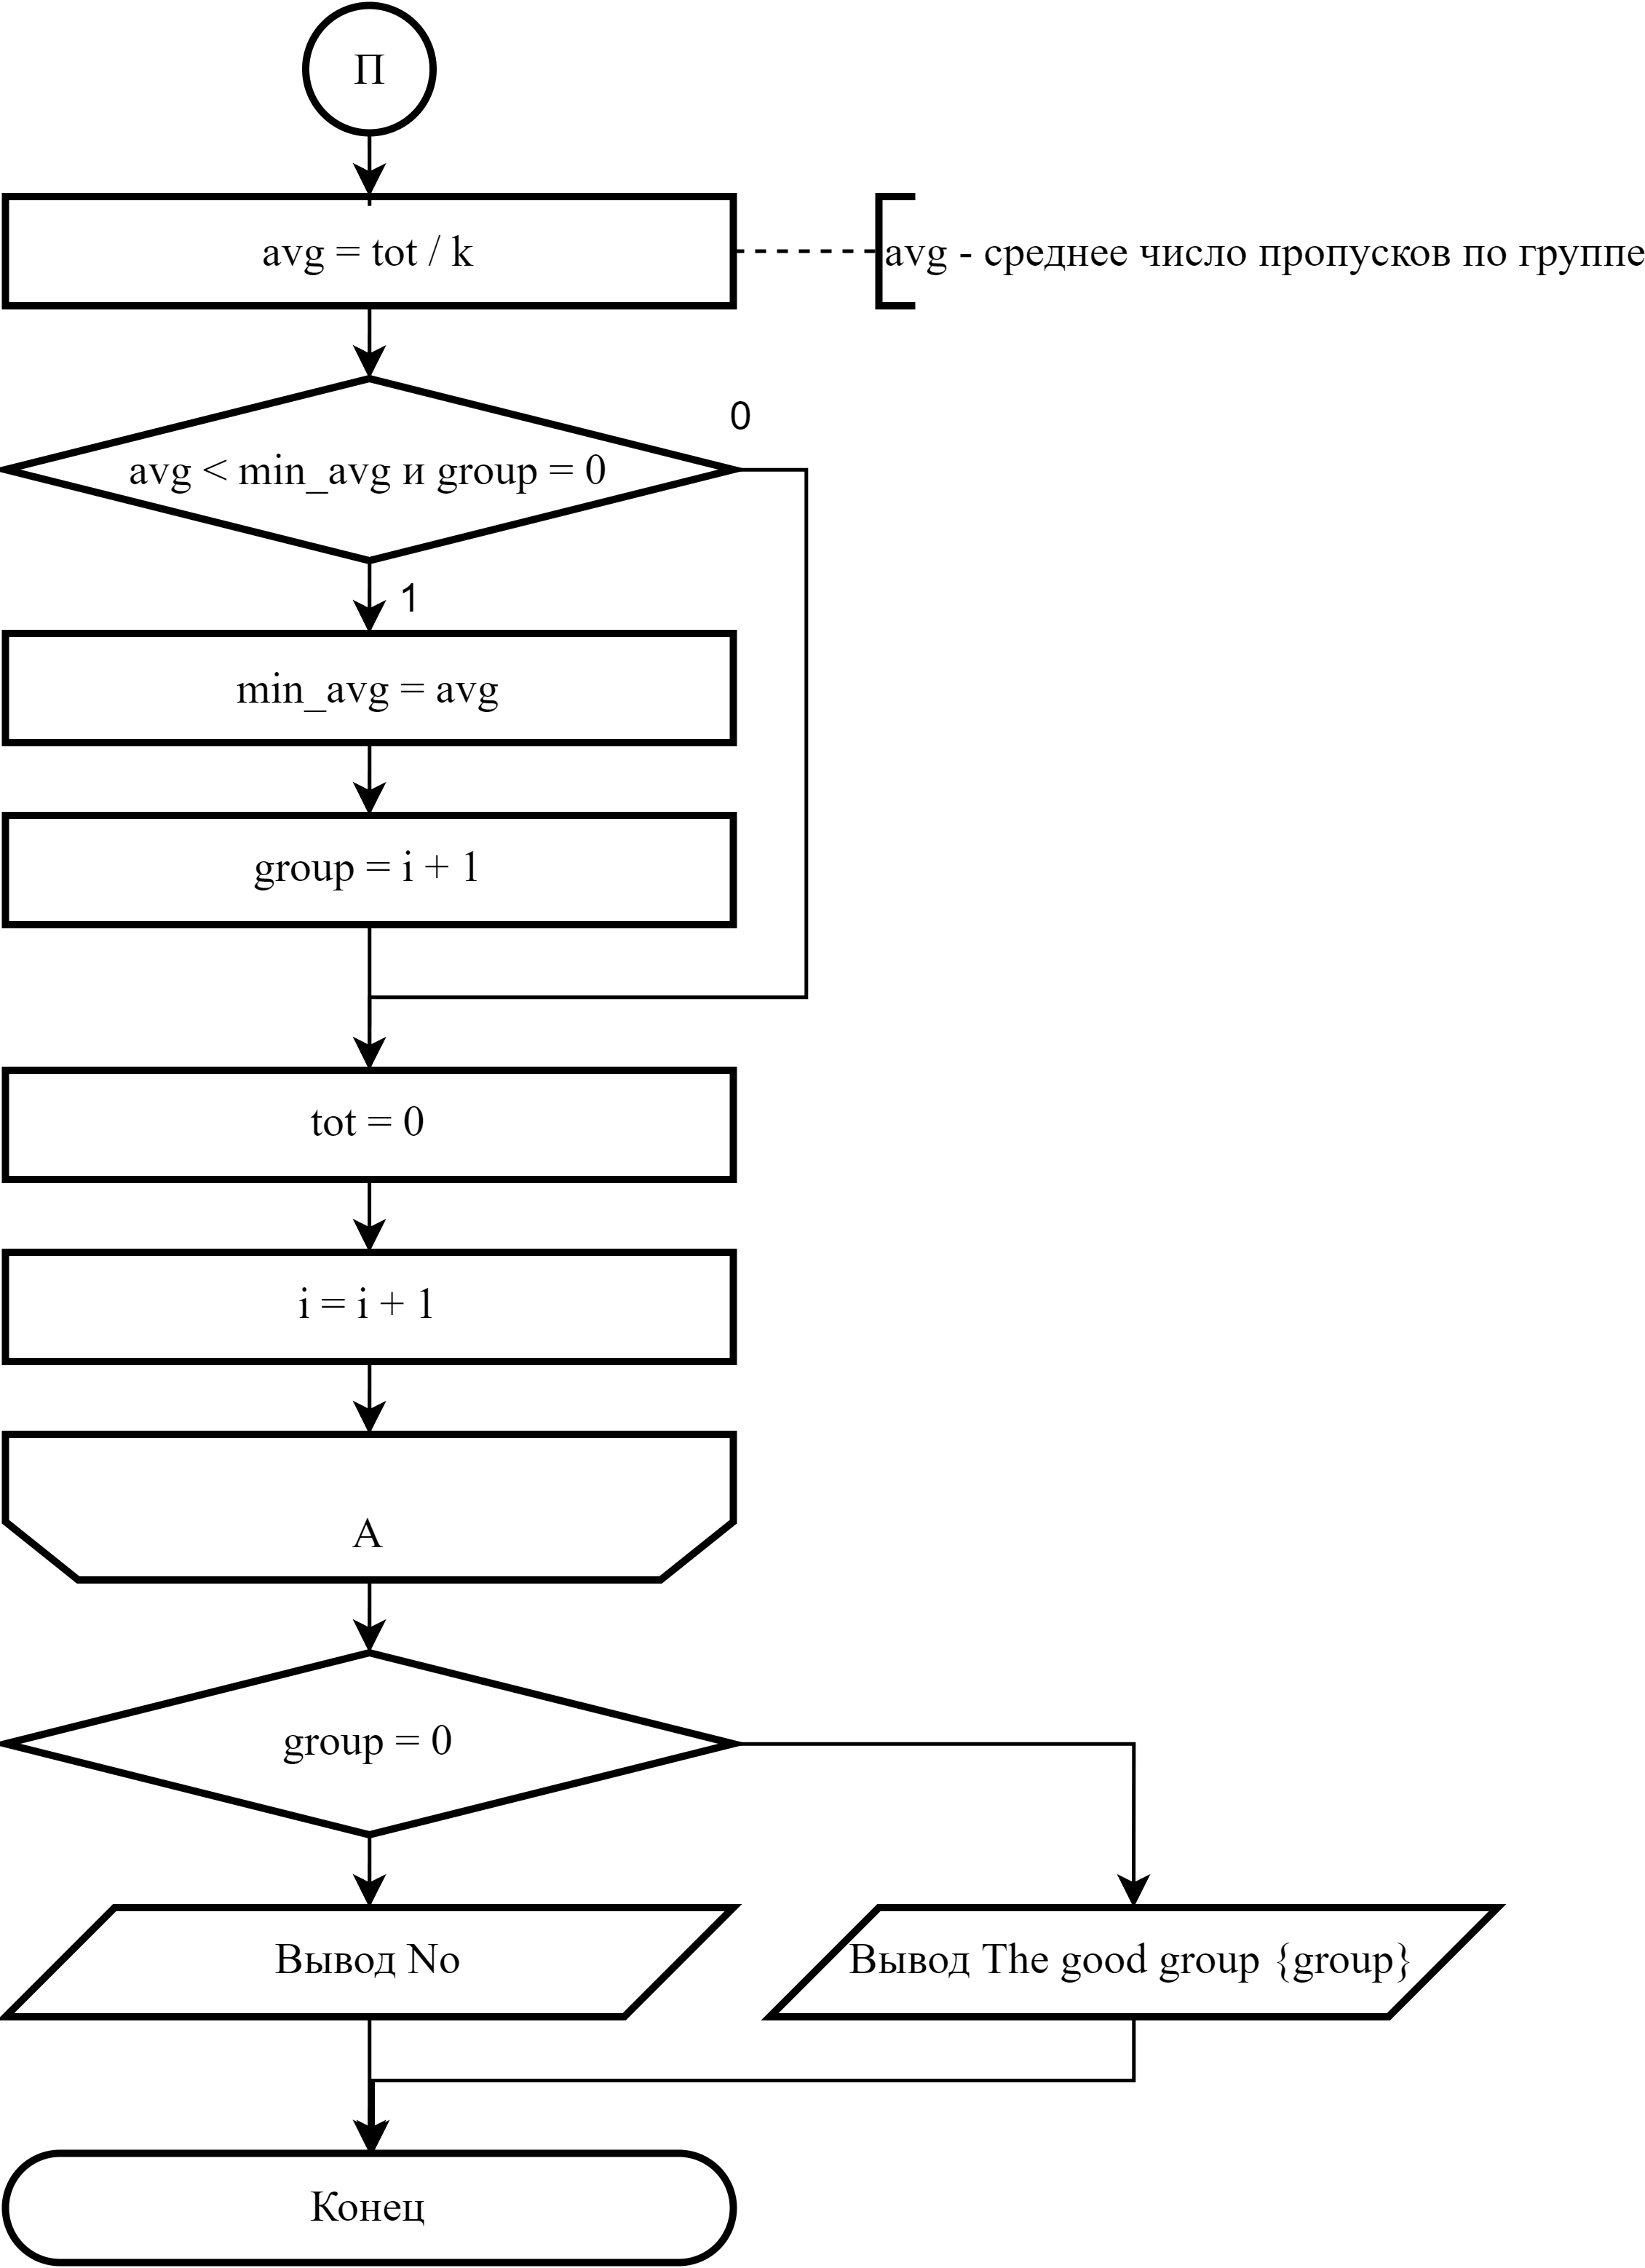
\includegraphics[height=0.85\textheight]{img/10-scheme-p2.png} % Укажите путь к изображению
	\caption{Схема алгоритма решения Задания 10.} % Подпись к изображению
\end{figure}
\begin{figure}
	\centering
	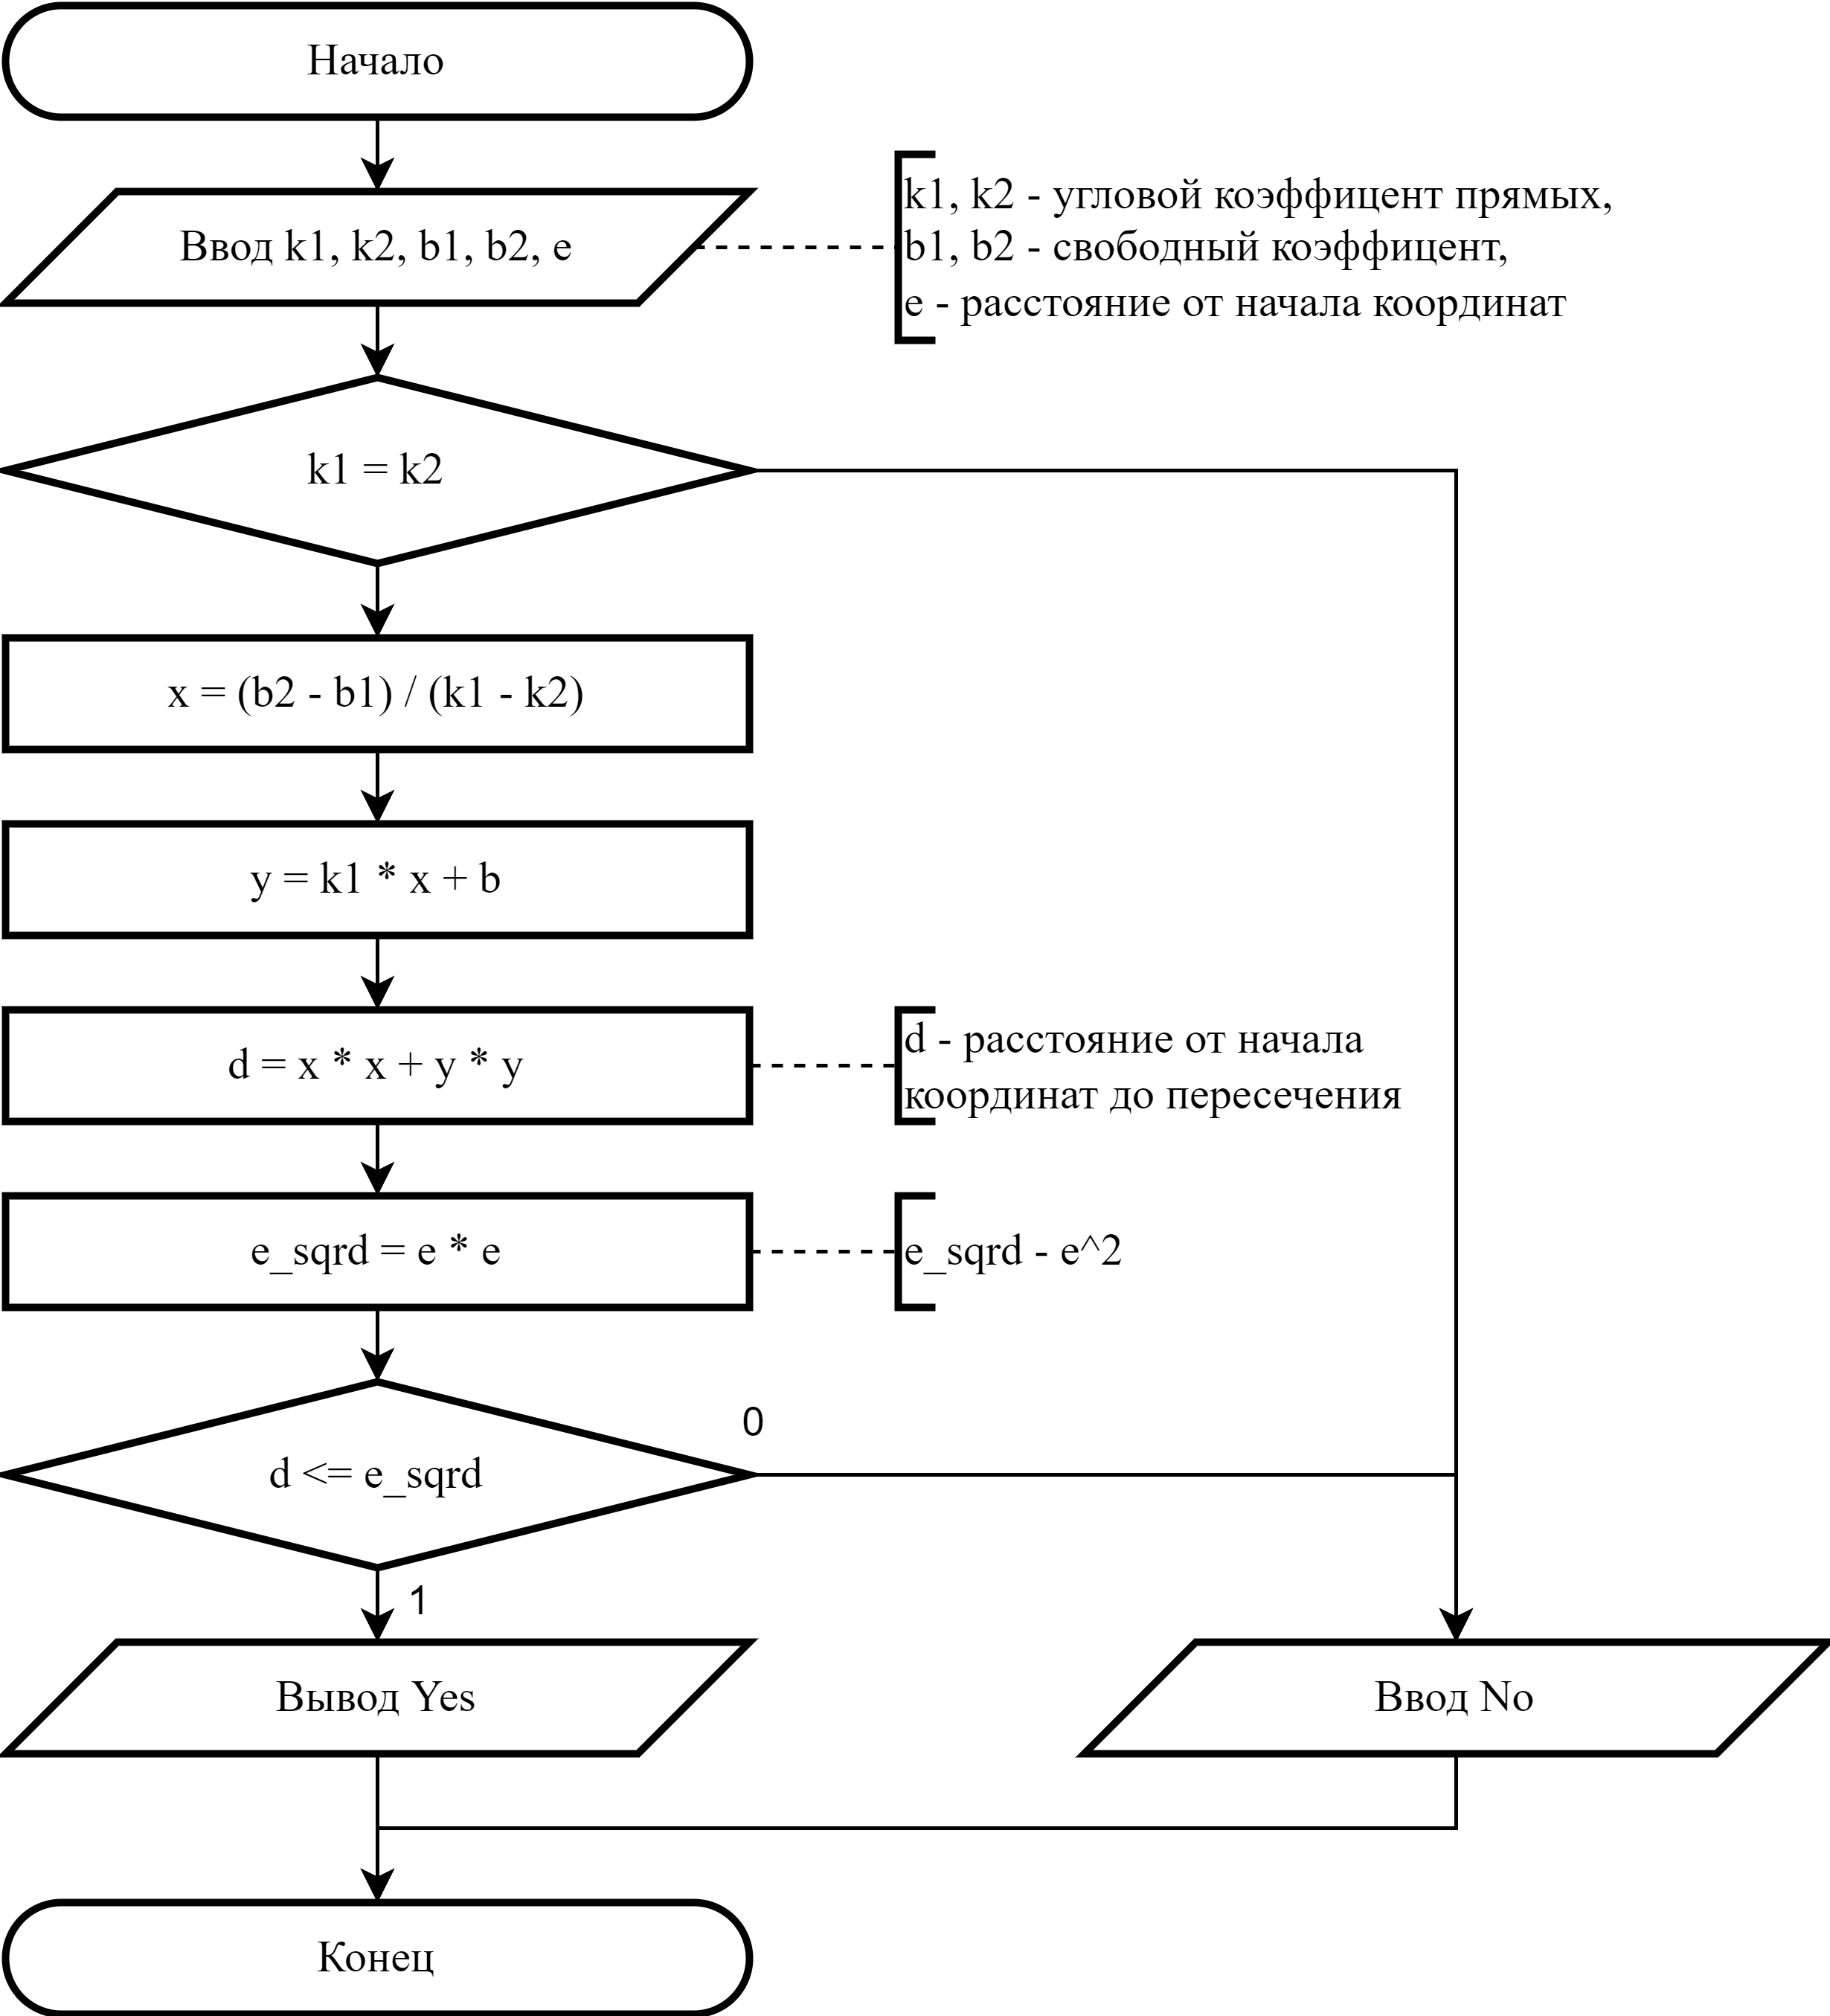
\includegraphics[width=0.95\textwidth]{img/11-scheme.png} % Укажите путь к изображению
	\caption{Схема алгоритма решения Задания 11.} % Подпись к изображению
\end{figure}
\begin{figure}
	\centering
	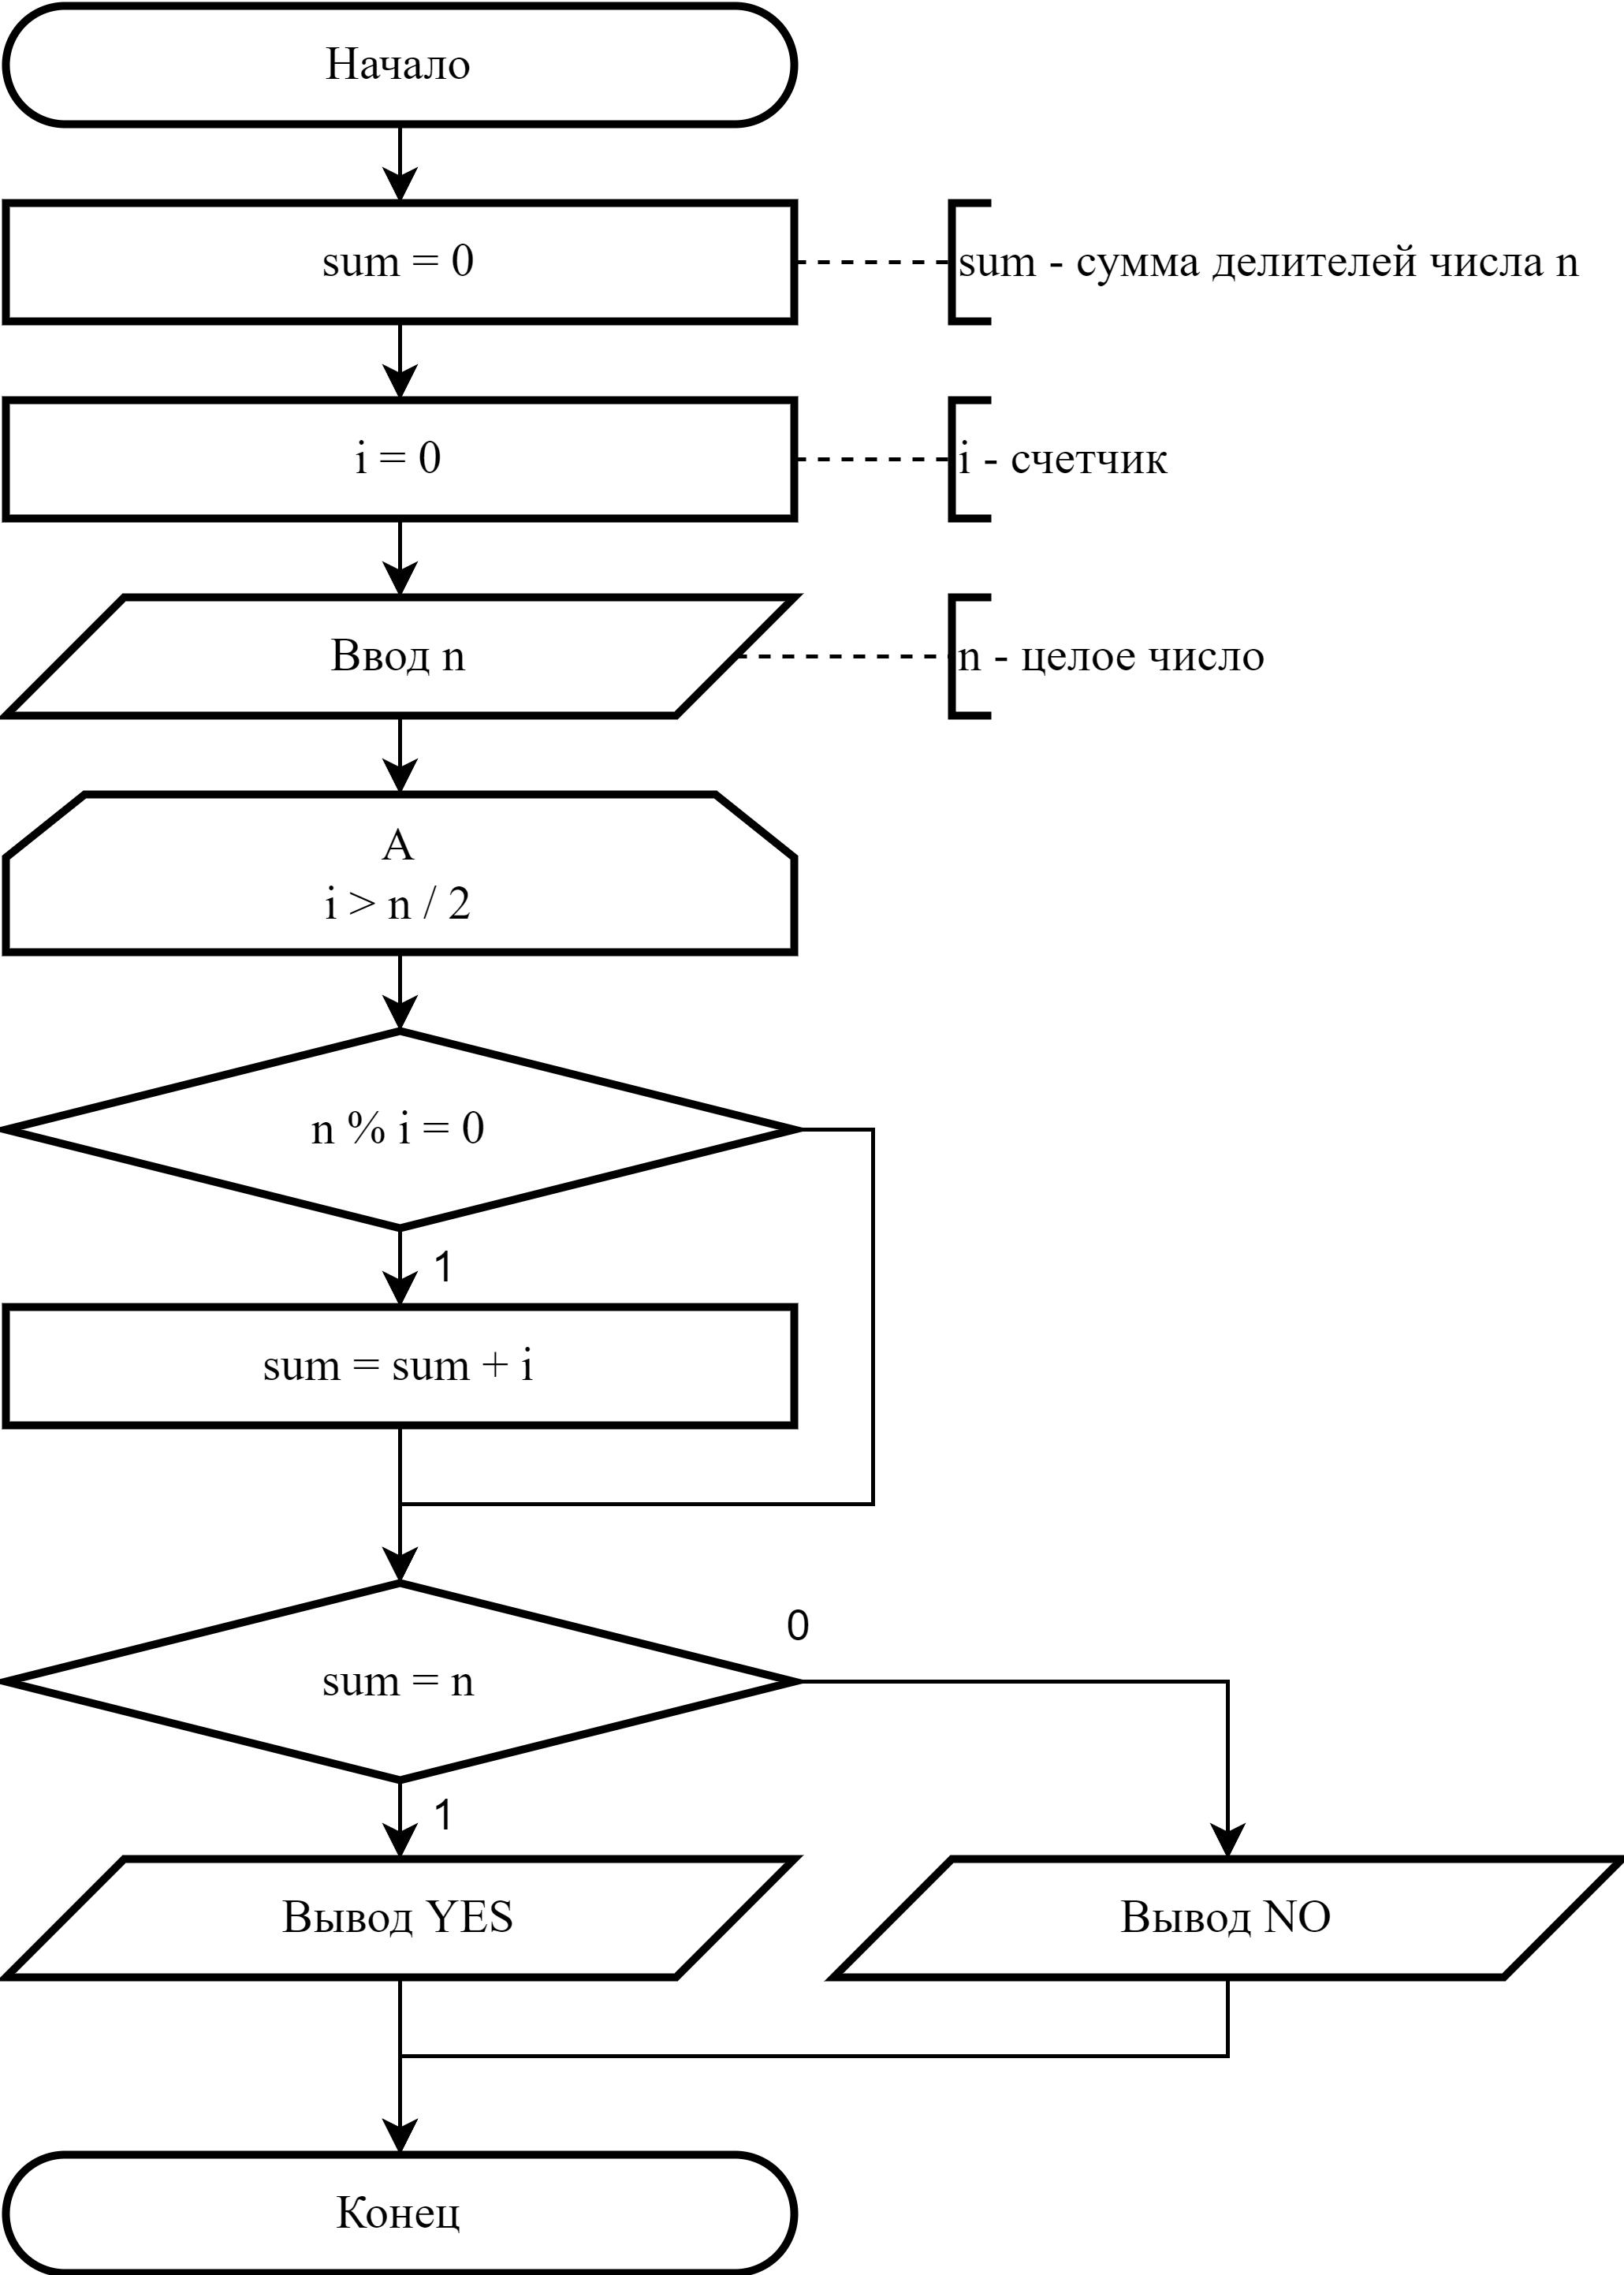
\includegraphics[height=0.9\textheight]{img/12-scheme.png} % Укажите путь к изображению
	\caption{Схема алгоритма решения Задания 12.} % Подпись к изображению
\end{figure}
\end{document}